%!TEX program = xelatex
%!TEX encoding = ISO-8859-1
\documentclass[12pt]{report}
\usepackage{caption}
\usepackage{amssymb}
\usepackage{amsmath,amsfonts,amsthm,amstext}
\usepackage[brazil]{babel}
% \usepackage[latin1]{inputenc}
\usepackage{graphicx}
\graphicspath{{/home/jfreitas/GitHub/Emural_Moodle/imagens/}}
\usepackage{enumerate}
\usepackage{hyperref}
\usepackage{float}
\usepackage{fancyhdr}

\def\ano{2022}
\def\semestre{2}
% \setlength{\topmargin}{-1.0in}
% \setlength{\oddsidemargin}{0in}
% \setlength{\textheight}{10.1in}
% \setlength{\textwidth}{6.5in}
% \setlength{\baselineskip}{12mm}

\pagestyle{fancy}

\begin{document}

\begin{center}
{\Large \textbf{Tutorial para a realiza\c{c}\~ao de backup de disciplinas no MoodleMAT}}
\end{center}
\vspace{.3cm}
\hrule

\vspace{.7cm}

Para efetuar o backup de uma disciplina no MoodleMAT os passos s\~ao os seguintes: acesse o MoodleMAT do ano e semestre que deseja realizar
o backup atrav\'es do endere\c{c}o \textit{https://moodle.mat.unb.br/anosemestre}, por exemplo, para fazer o backup da disciplina do
\ano/\semestre\ o endere\c{c}o seria \href{https://moodle.mat.unb.br/\ano\semestre}{https://moodle.mat.unb.br/\ano\semestre} (o endere\c{c}o \href{https://moodle.mat.unb.br}{https://moodle.mat.unb.br}, refere-se sempre ao semestre corrente).

\begin{enumerate}[\bf 1)]
    \item Ap\'os entrar na sua disciplina, no menu superior clique na opção ``\textbf{Mais}''.
	\begin{figure}[H]
    	\centering
    	\hspace*{-2.5cm}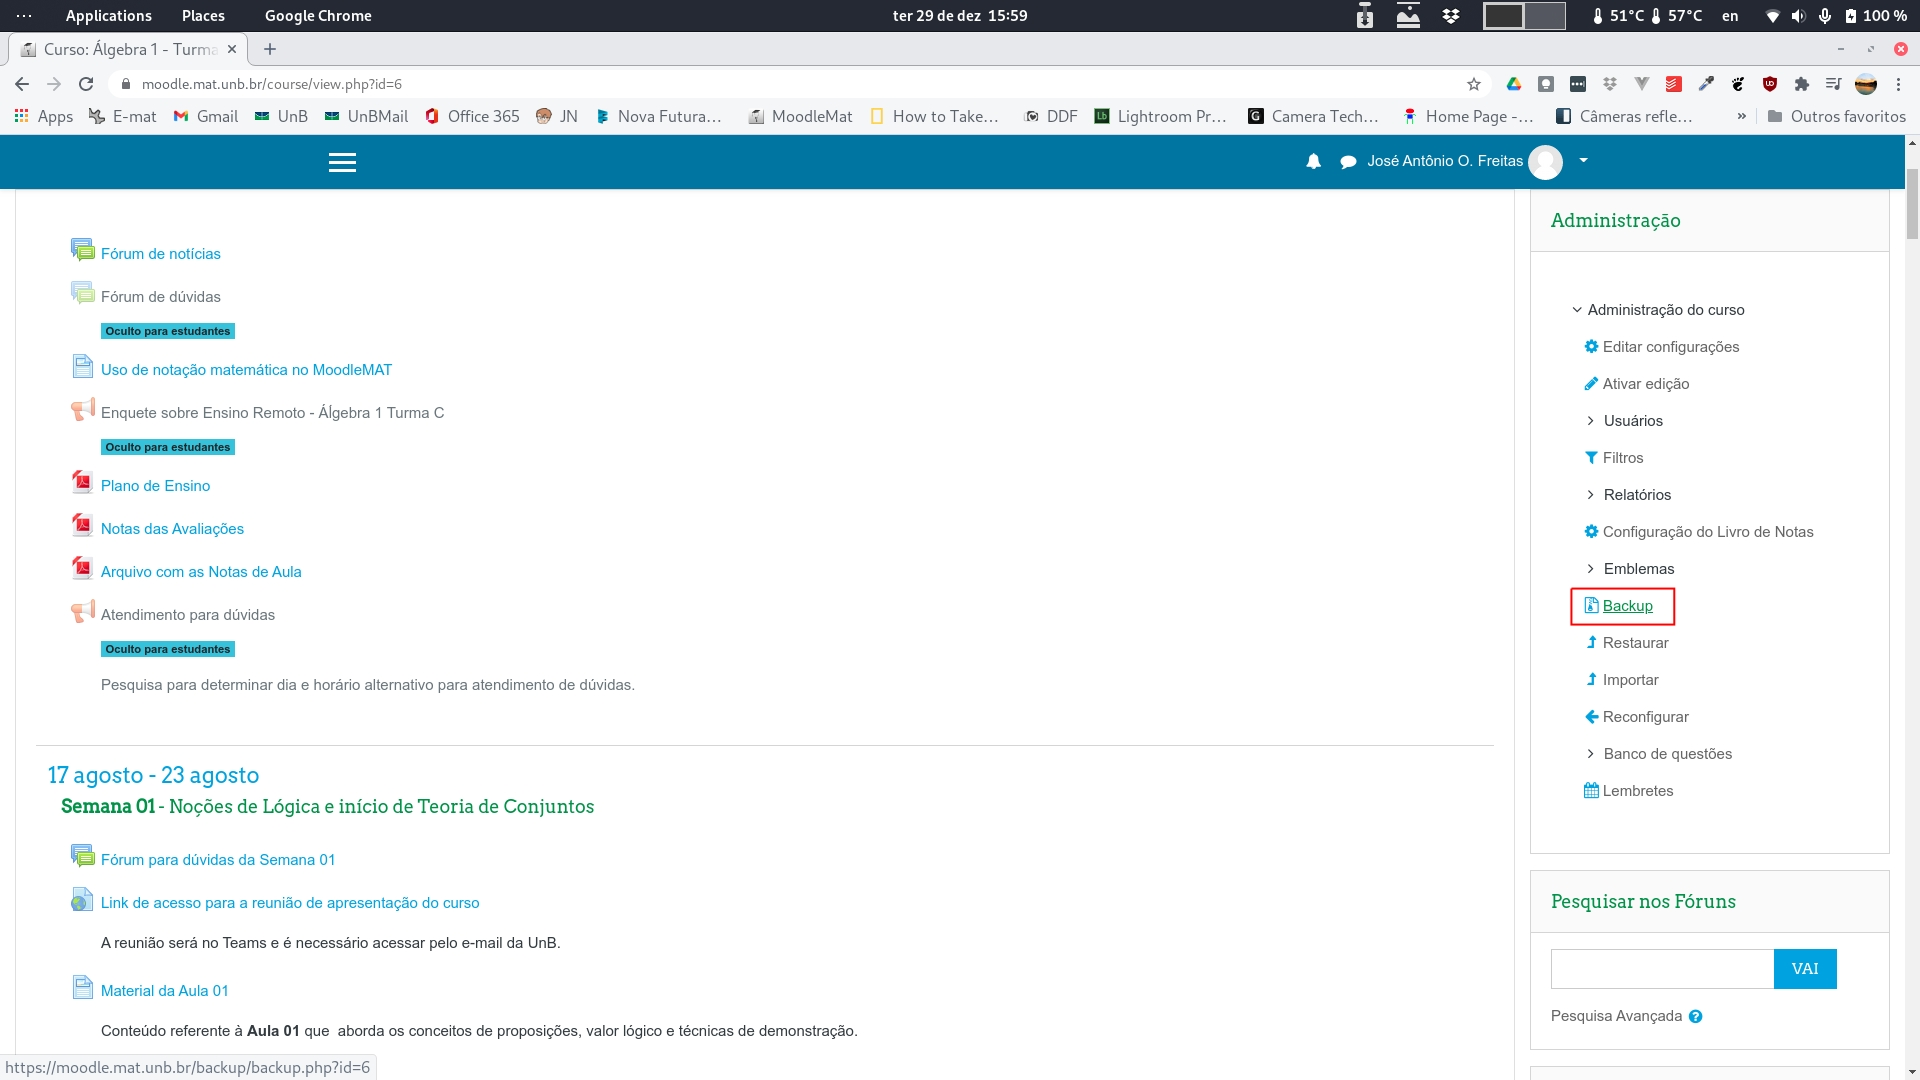
\includegraphics[width = 1.4\columnwidth]{tela_backup_1.jpg}
  	\end{figure}

	\newpage

        \item No menu que irá se abrir, procure a opção ``\textbf{Reutilizar curso}'' e clique nela.
	\begin{figure}[H]
	   \centering
        	\hspace*{-2.5cm}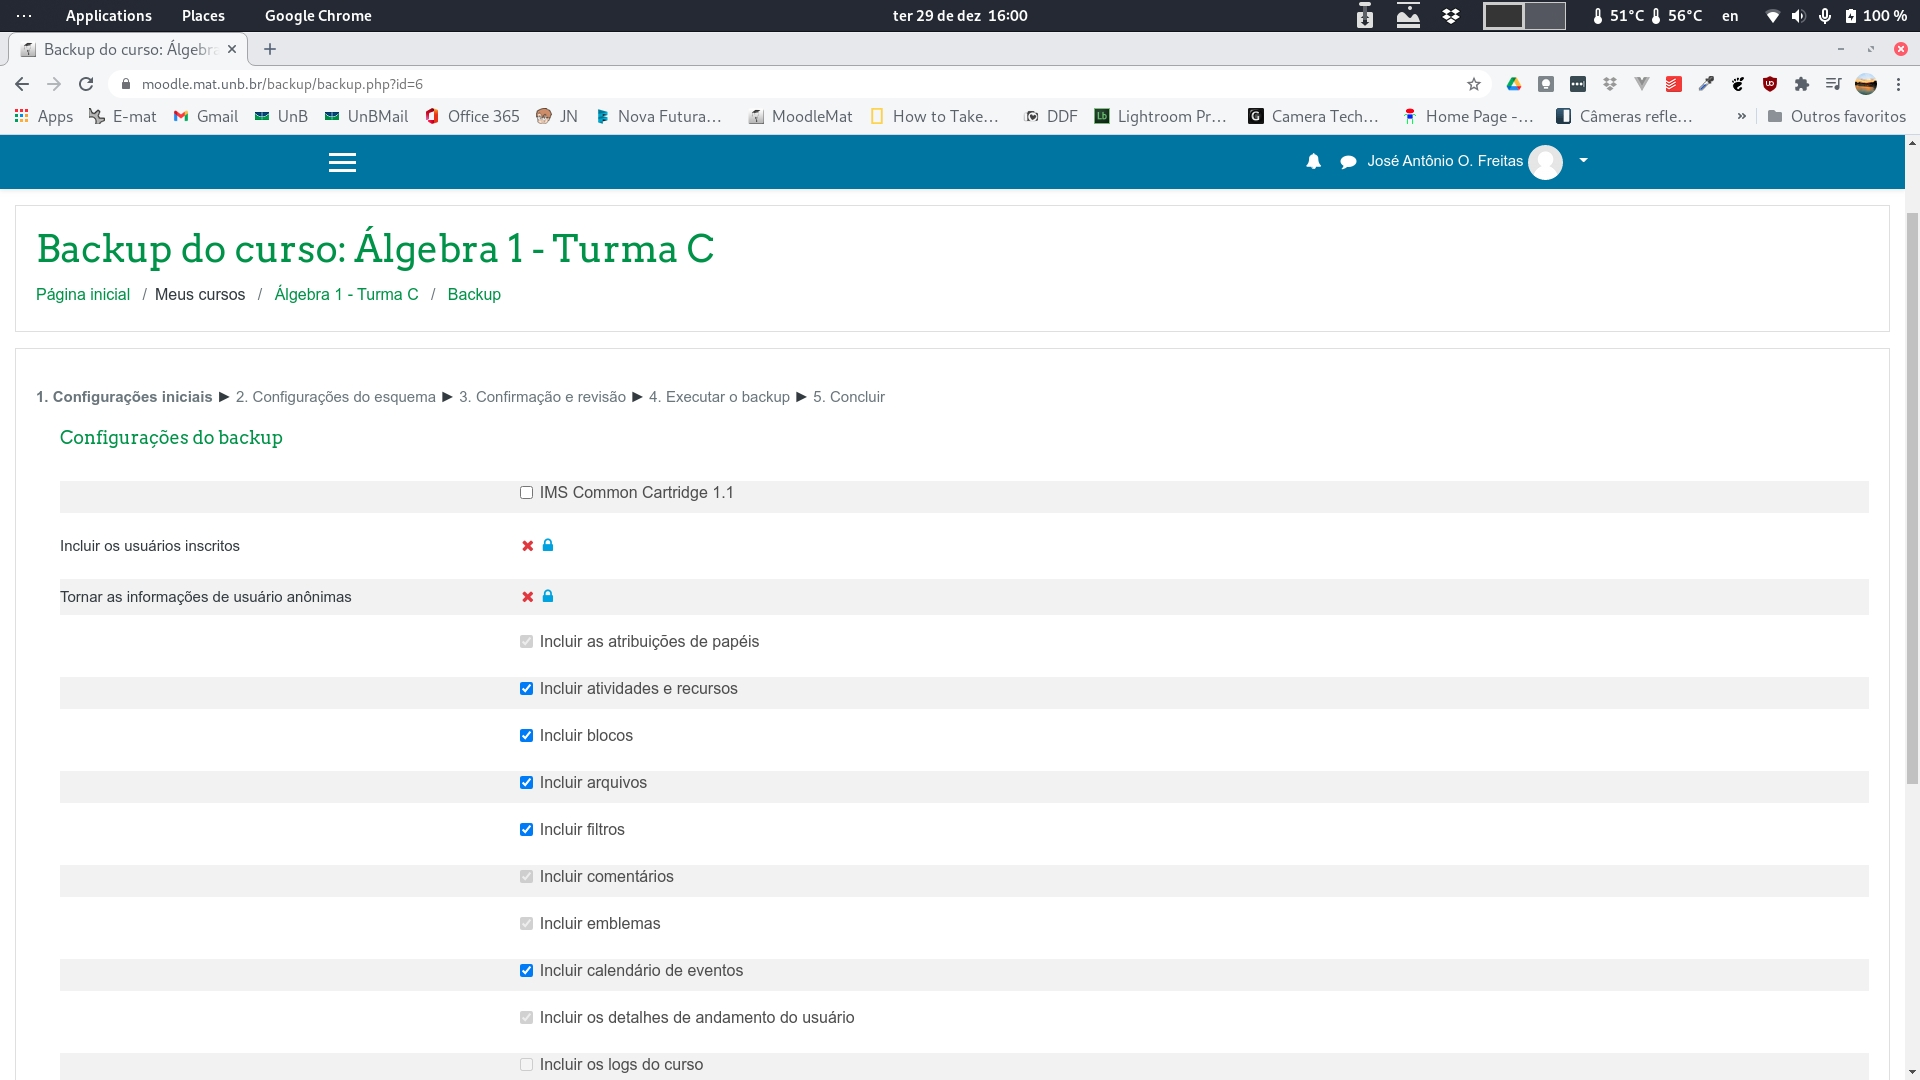
\includegraphics[width = 1.4\columnwidth]{tela_backup_2.jpg}
	    \end{figure}
	
	\newpage

	\item A tela seguinte, à sua esquerda, procure o texto "\textbf{Importar}" e clique nele. No menu que se abre escolha a opção ``\textbf{Backup}'' e clique nela.
	\begin{figure}[H]
    	\centering
    	\hspace*{-2.5cm}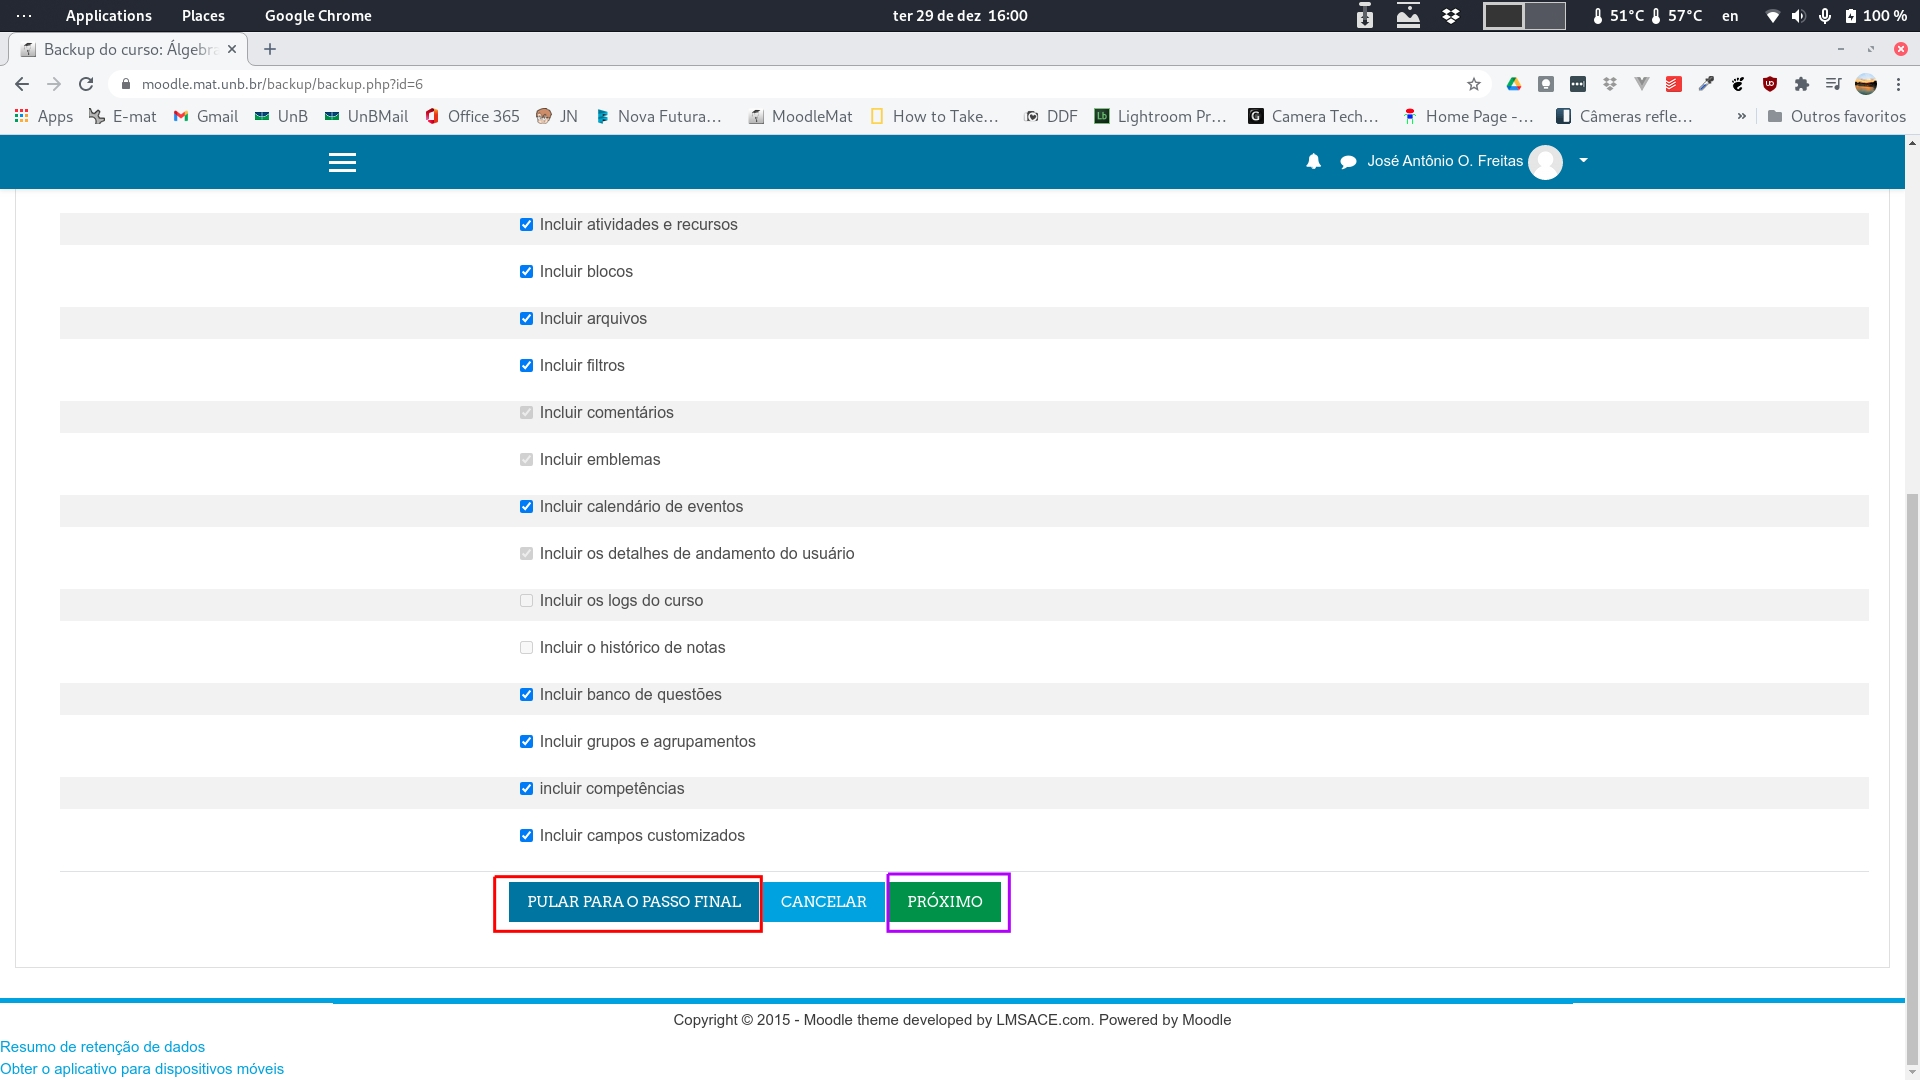
\includegraphics[width = 1.4\columnwidth]{tela_backup_3.jpg}
  	\end{figure}
	
	\begin{figure}[H]
    	\centering
    	\hspace*{-2.5cm}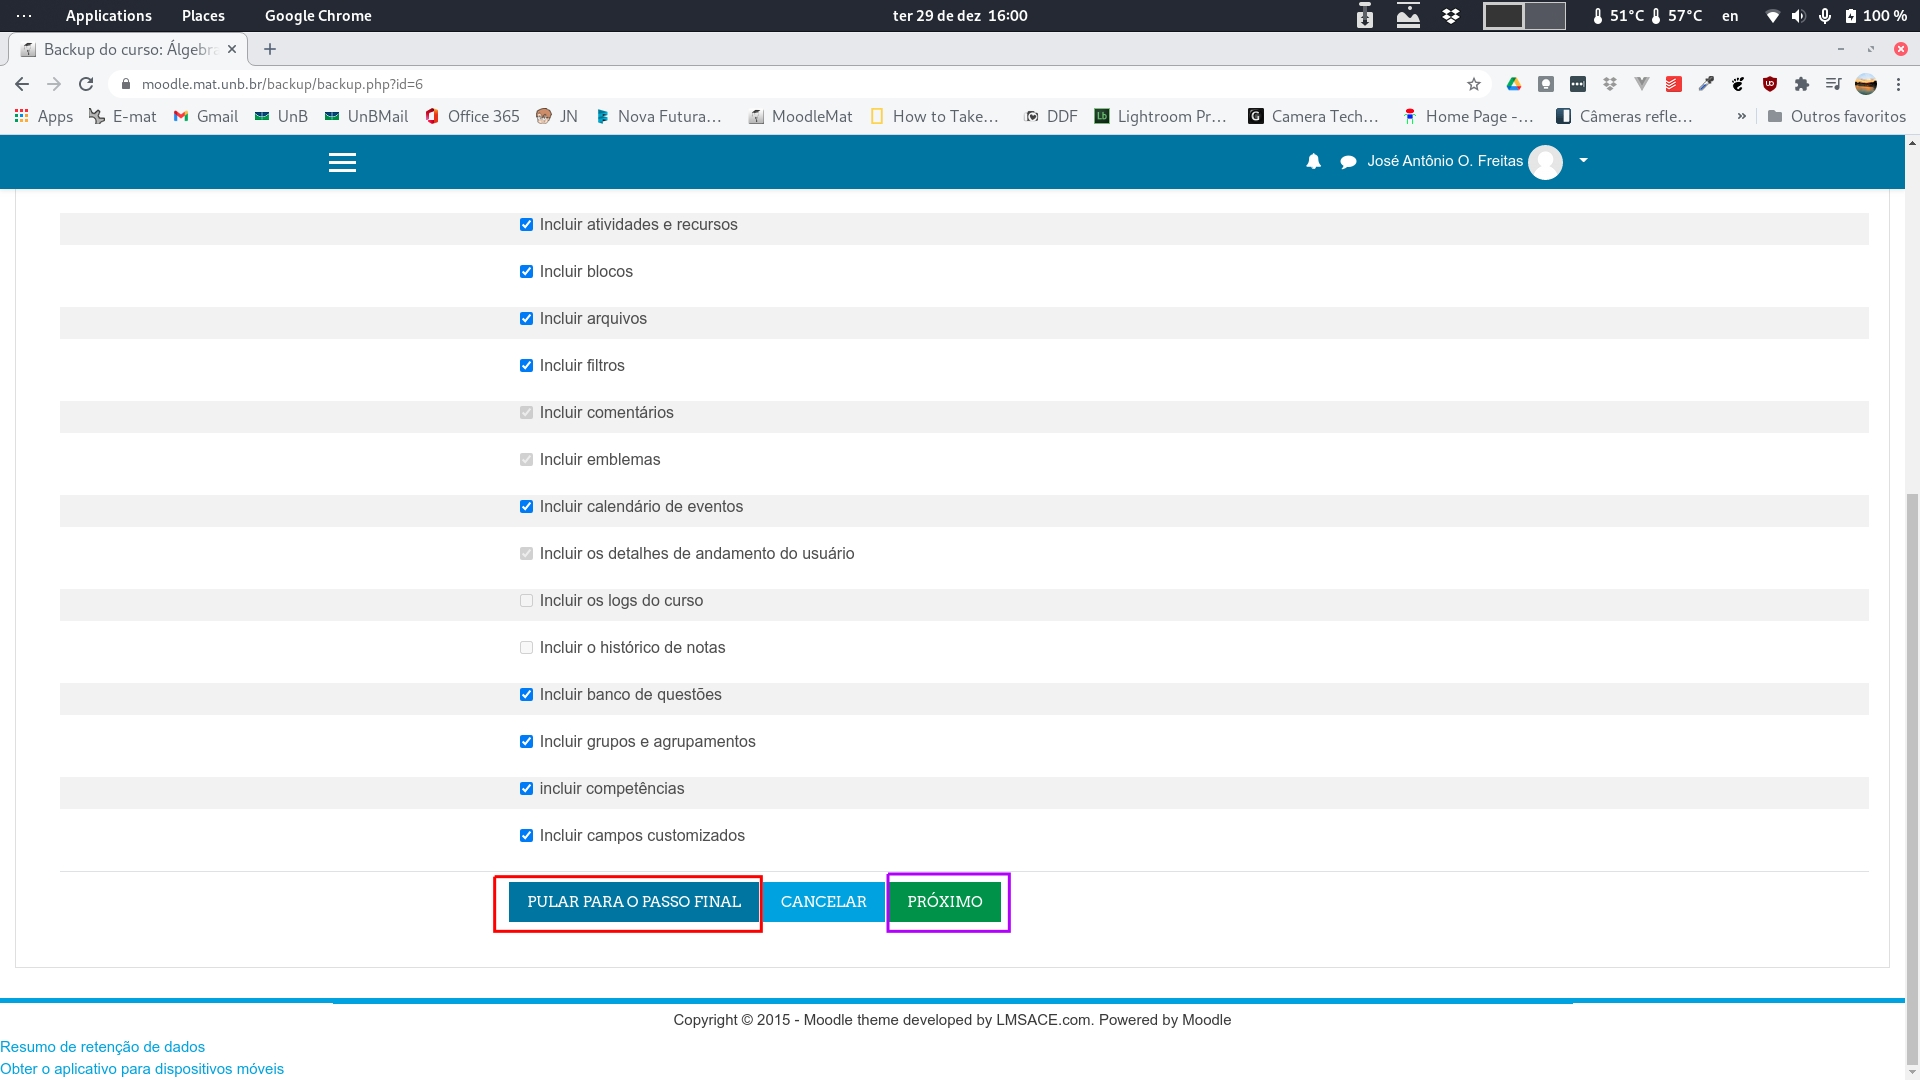
\includegraphics[width = 1.4\columnwidth]{tela_backup_3.jpg}
  	\end{figure}

  	\newpage

	\item Na tela que se abre, role a página at\'e o final onde ser\~ao apresentadas as op\c{c}\~oes: ``PULAR PARA O PASSO FINAL'' e ``PR\'OXIMO''. O MoodleMAT \textbf{j\'a est\'a configurado} para salvar somente os dados importantes das disciplinas de modo que \'e \textbf{recomendando} utilizar a op\c{c}\~ao ``PULAR PARA O PASSO FINAL". Mas caso algu\'em deseje revisar as op\c{c}\~oes ou alterar algum dado que ser\'a salvo dever\'a utilizar a op\c{c}\~ao ``PR\'OXIMO''.
	\begin{figure}[H]
    	\centering
    	\hspace*{-2.5cm}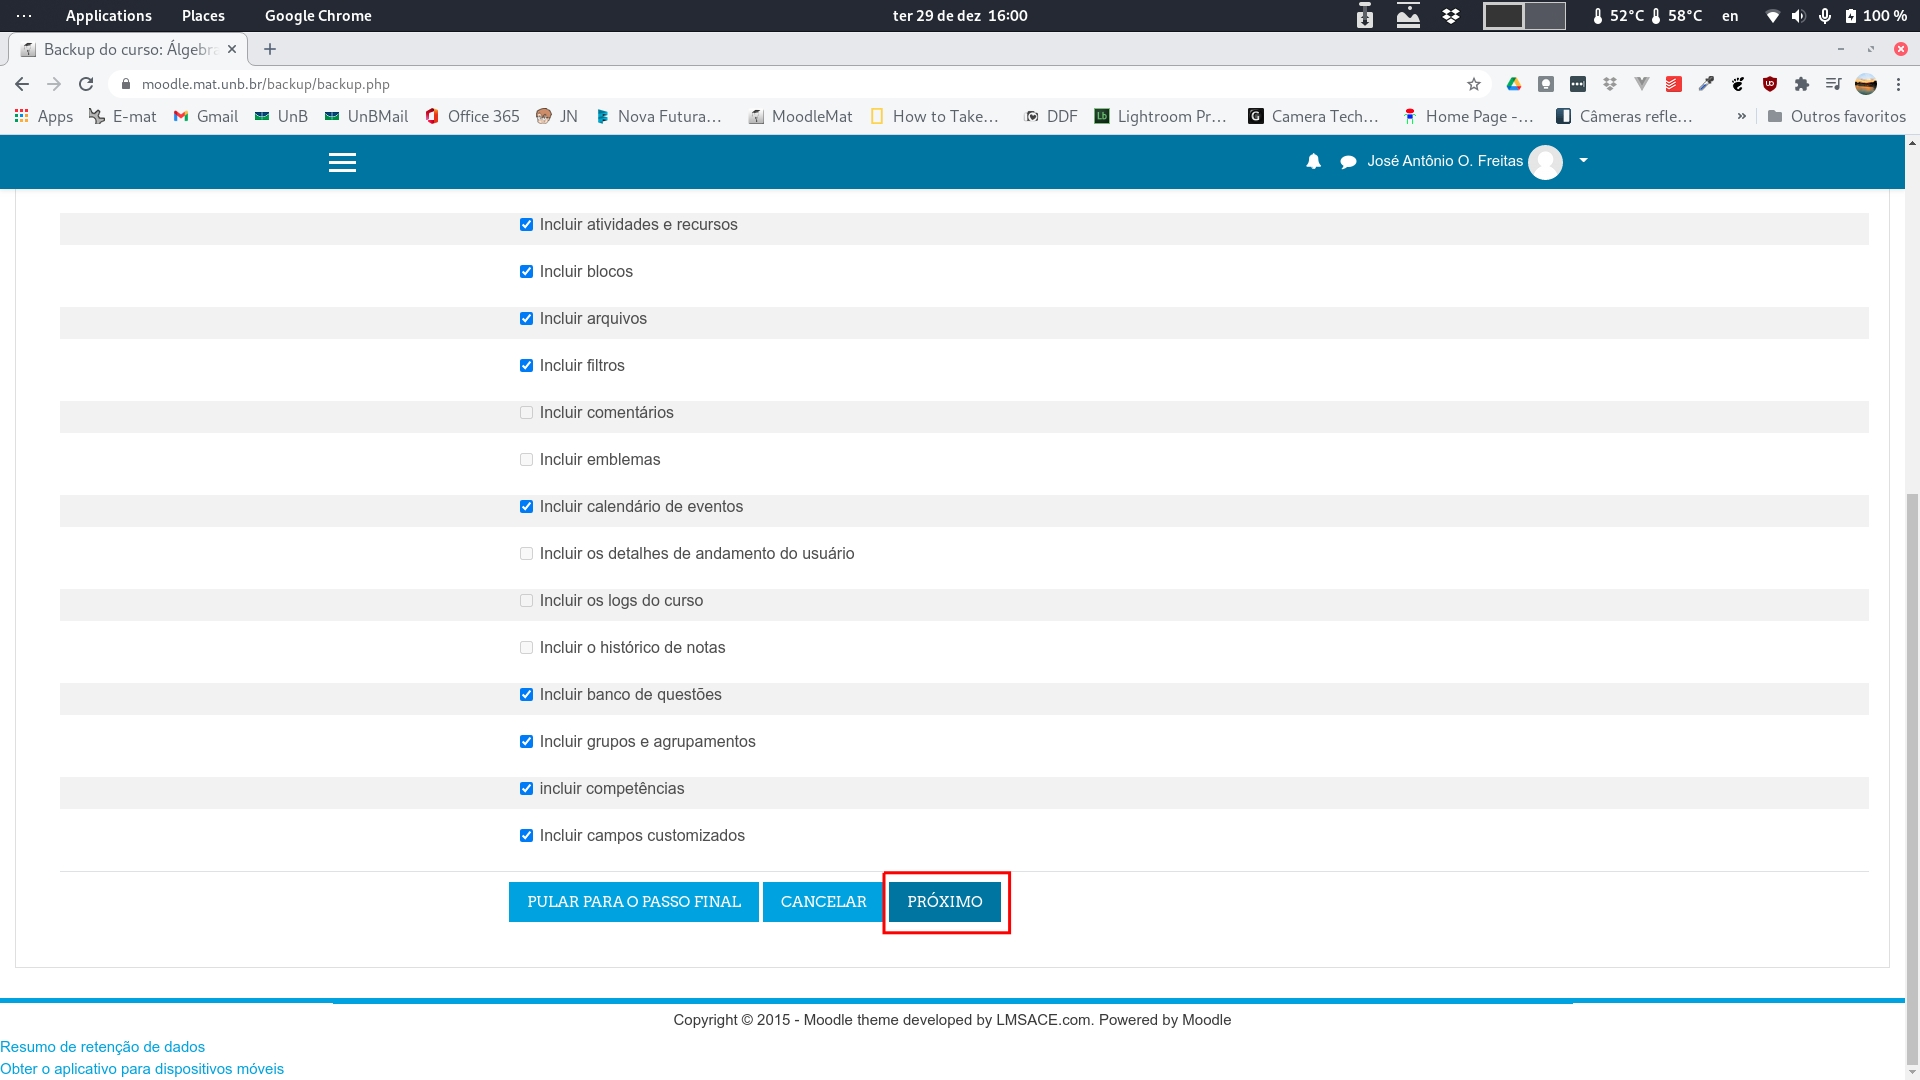
\includegraphics[width = 1.4\columnwidth]{tela_backup_4.jpg}
  	\end{figure}

  	\newpage

	\item Caso escolha a op\c{c}\~ao ``PULAR PARA O PASSO FINAL" o backup ser\'a iniciado, o processo pode ser um pouco demorado, dependendo da quantidade de recursos da disciplina.
	\begin{figure}[H]
    	\centering
    	\hspace*{-2.5cm}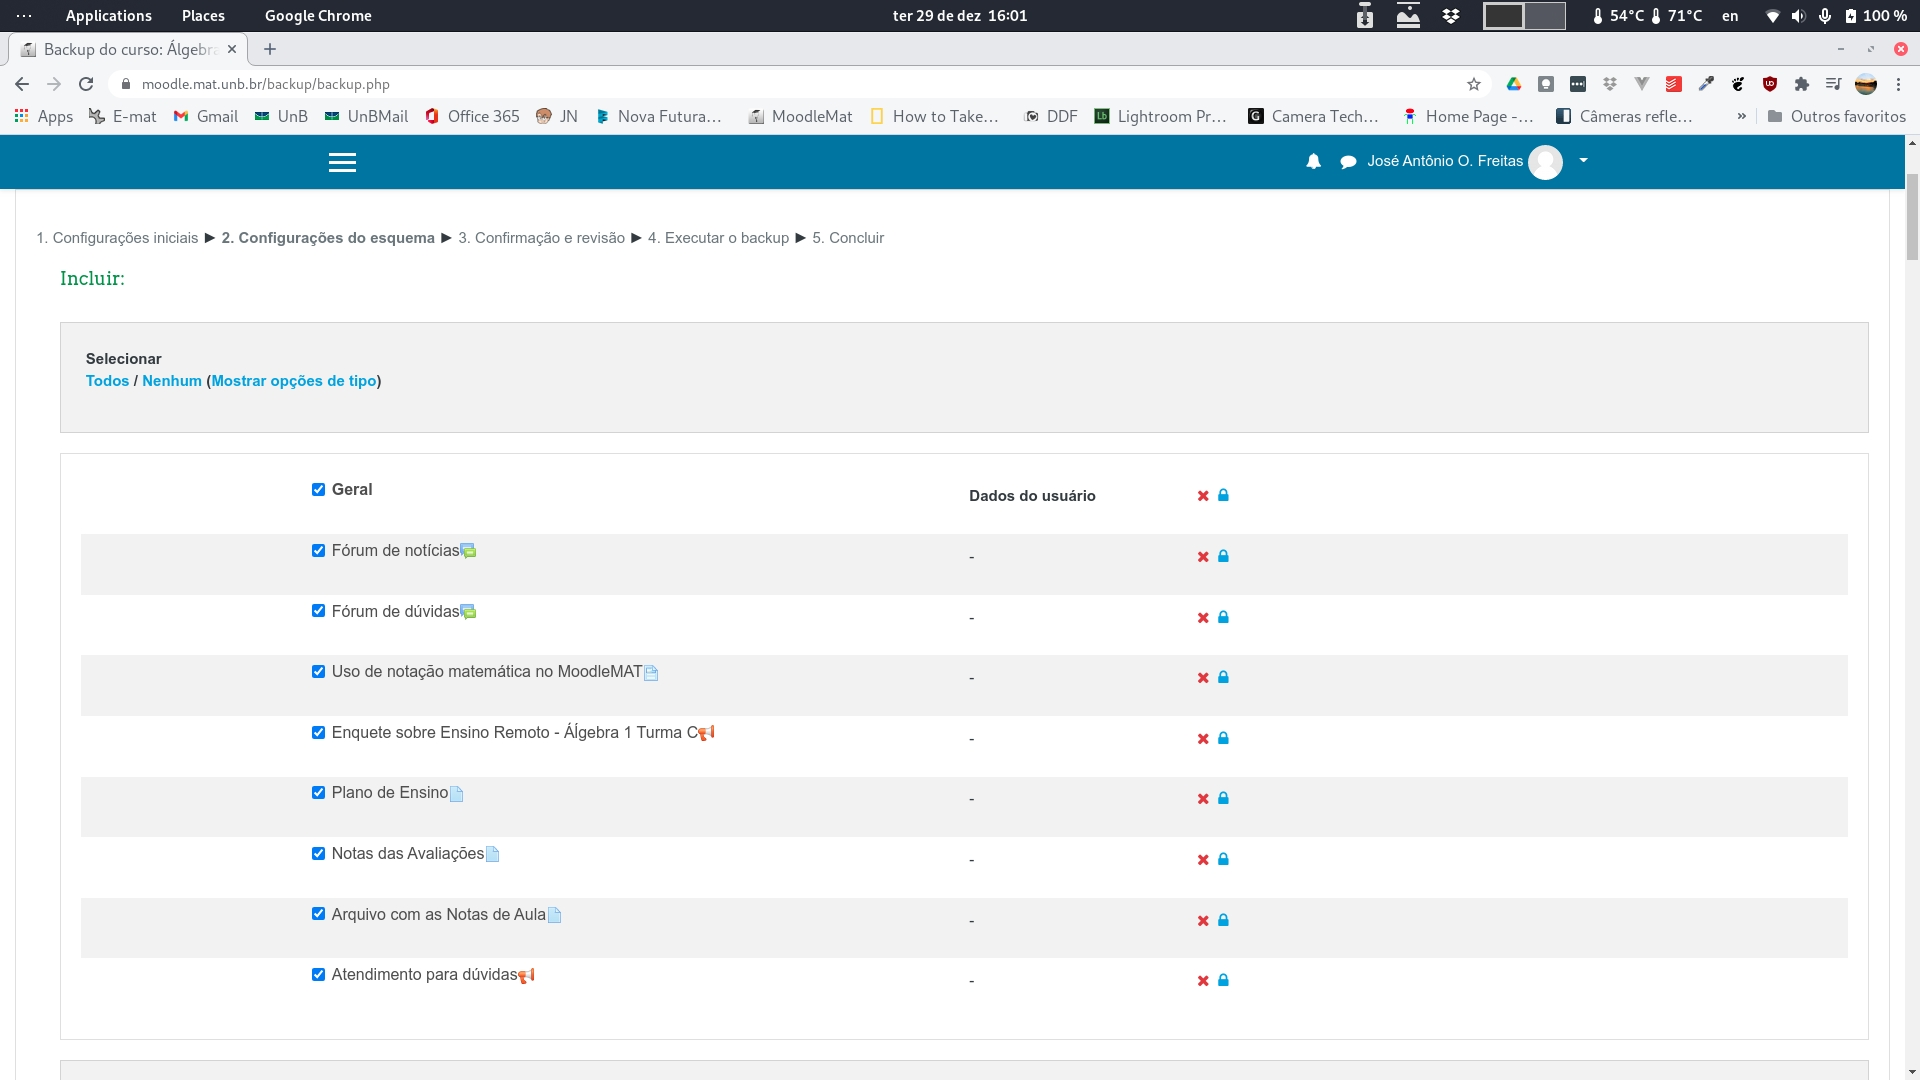
\includegraphics[width = 1.4\columnwidth]{tela_backup_6.jpg}
  	\end{figure}

        \item Ao final do processo você será levado para a tela mostrada no \textbf{item \ref{final_backup}}.
  	\newpage

	\item Caso escolha a op\c{c}\~ao ``PR\'OXIMO'', voc\^e ser\'a direcionando \`a pr\'oxima tela na qual ser\'a alterar algumas configura\c{c}\~oes do backup.
	\begin{figure}[H]
    	\centering
    	\hspace*{-2.5cm}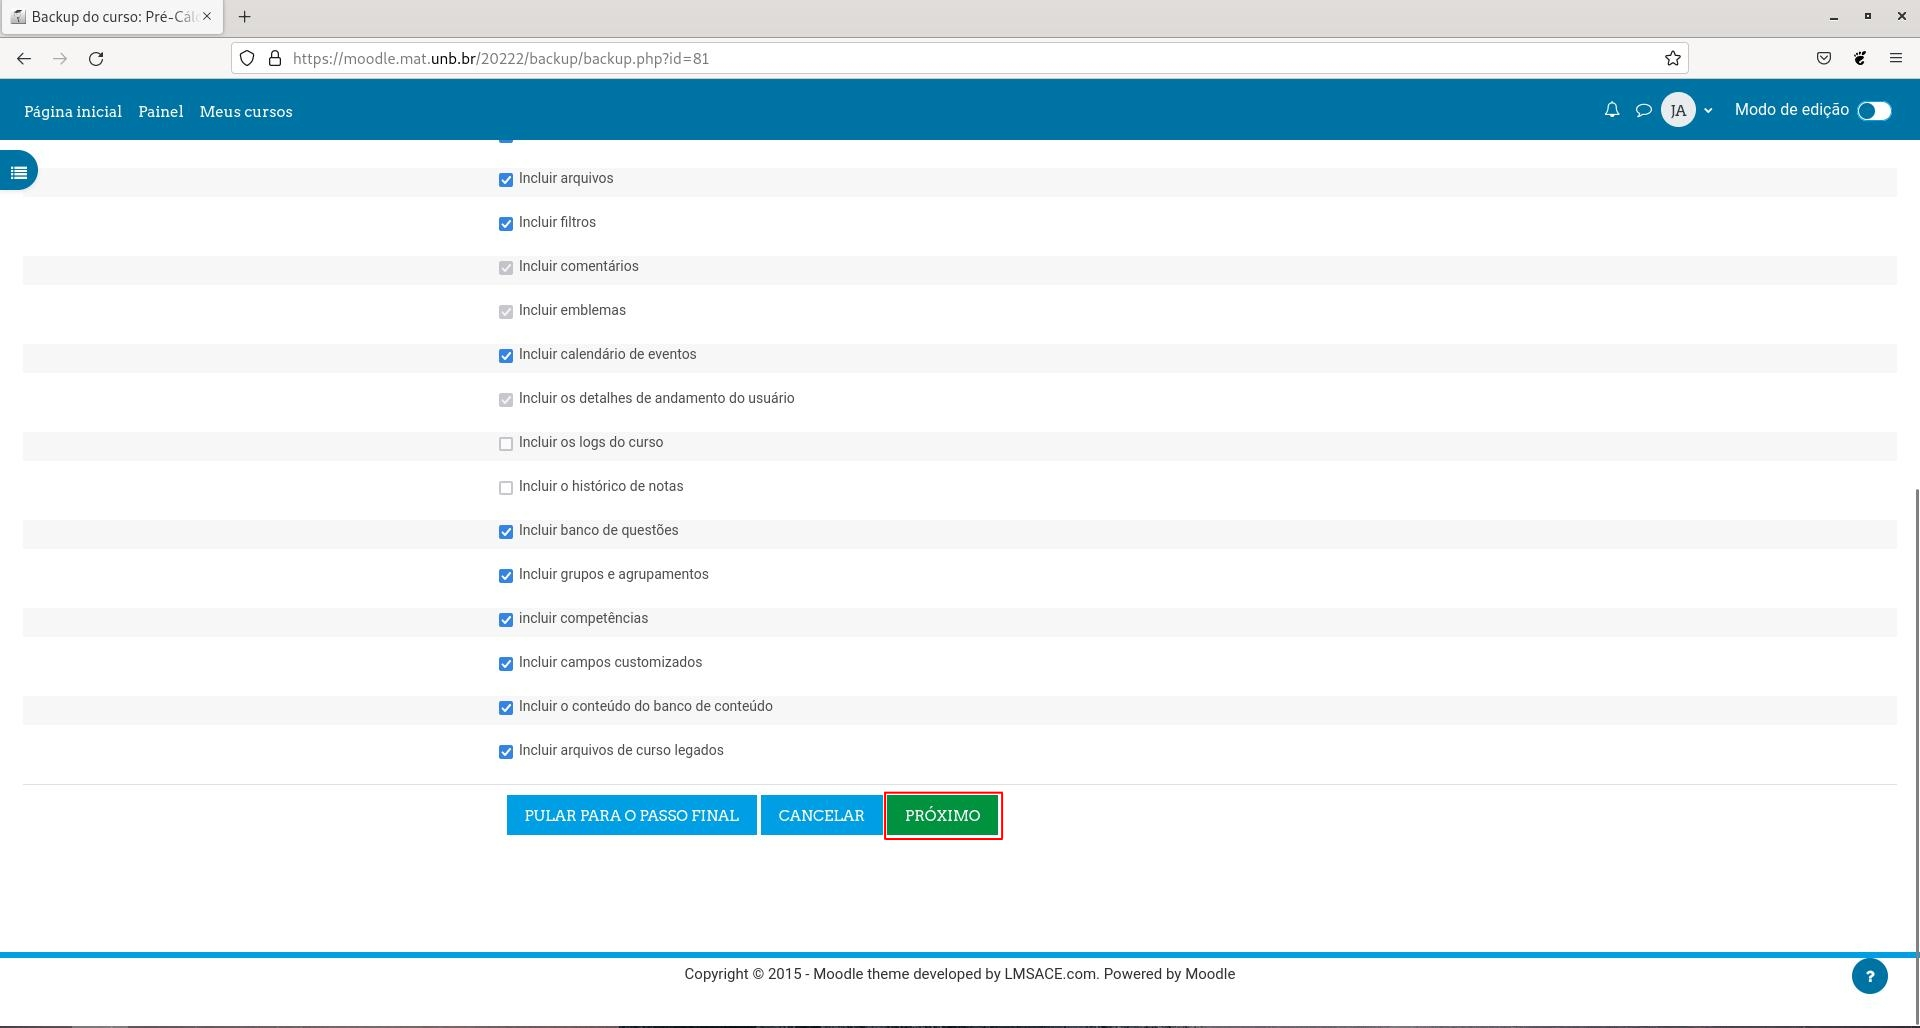
\includegraphics[width = 1.4\columnwidth]{tela_backup_7.jpg}
  	\end{figure}

  	\newpage

	\item Nas pr\'oximas telas ser\~ao apresentadas algumas configura\c{c}\~oes do backup que podem ser alteradas. Mude aquelas que desejar e role a tela at\'e o final para encontrar o bot\~ao ``PR\'OXIMO''.
	\begin{figure}[H]
    	\centering
    	\hspace*{-2.5cm}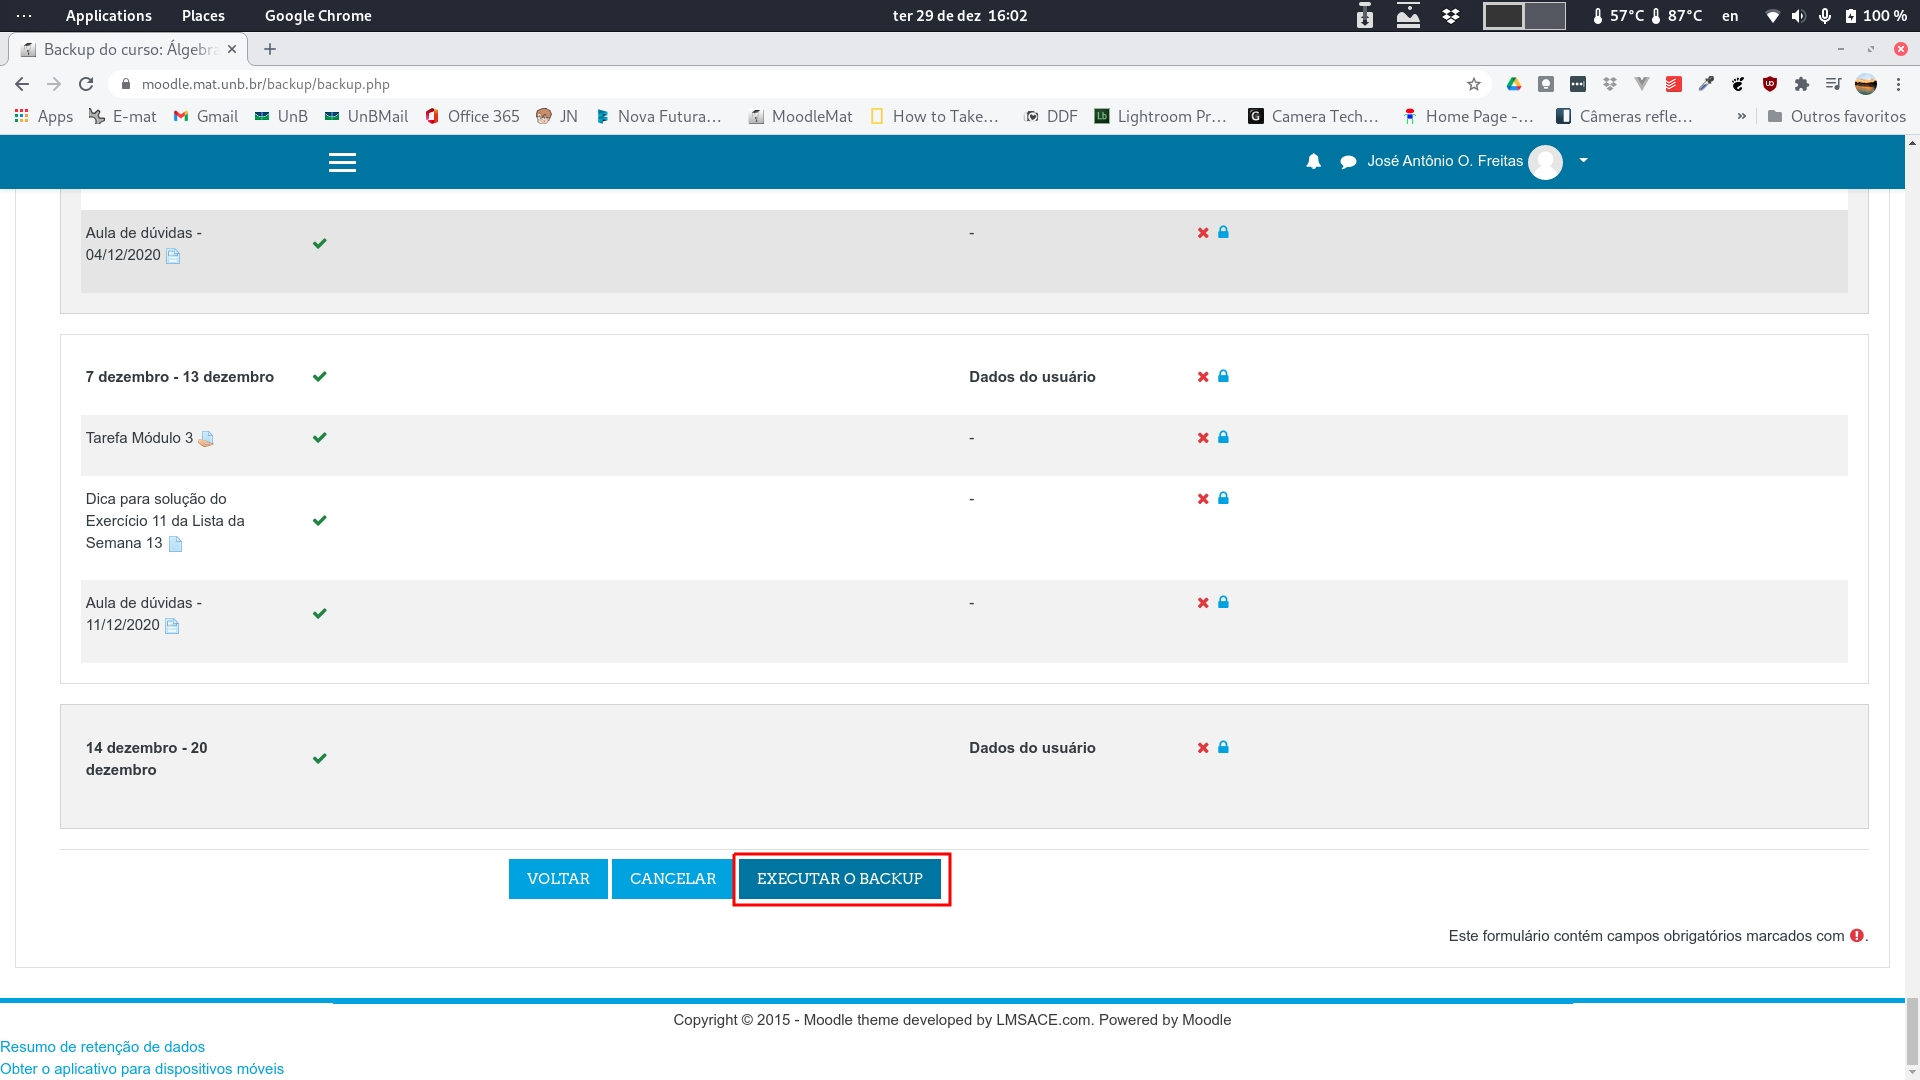
\includegraphics[width = 1.4\columnwidth]{tela_backup_8.jpg}
  	\end{figure}

  	\newpage

        \item Ao final da tela seguinte você encontrará o botão ``\textbf{EXECUTAR O BACKUP}''. Clique nele para o backup seja executado.
	\begin{figure}[H]
    	\centering
    	\hspace*{-2.5cm}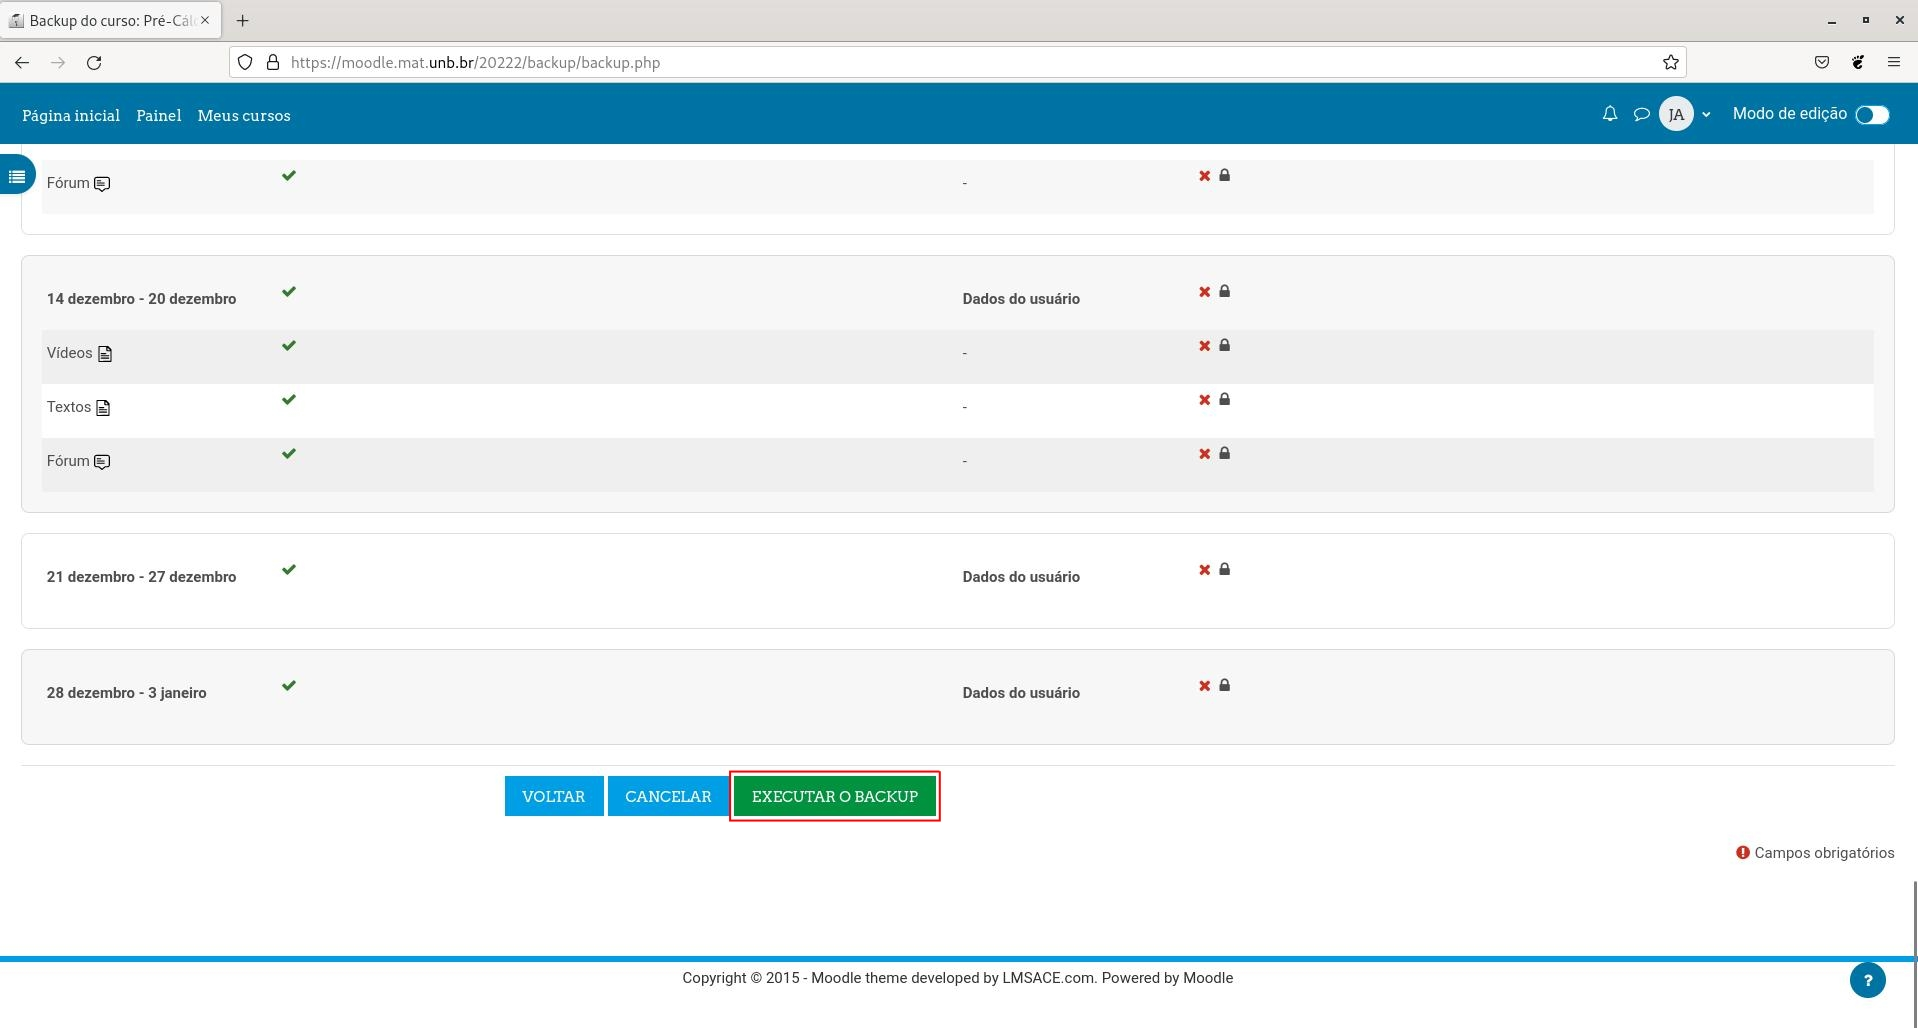
\includegraphics[width = 1.4\columnwidth]{tela_backup_9.jpg}
  	\end{figure}

	\newpage

        \item  Ao clicar no botão ``\textbf{EXECUTAR O BACKUP}'' o processo se inicia e pode ser um pouco demorado, dependendo da quantidade de recursos da disciplina.
	\begin{figure}[H]
    	\centering
    	\hspace*{-2.5cm}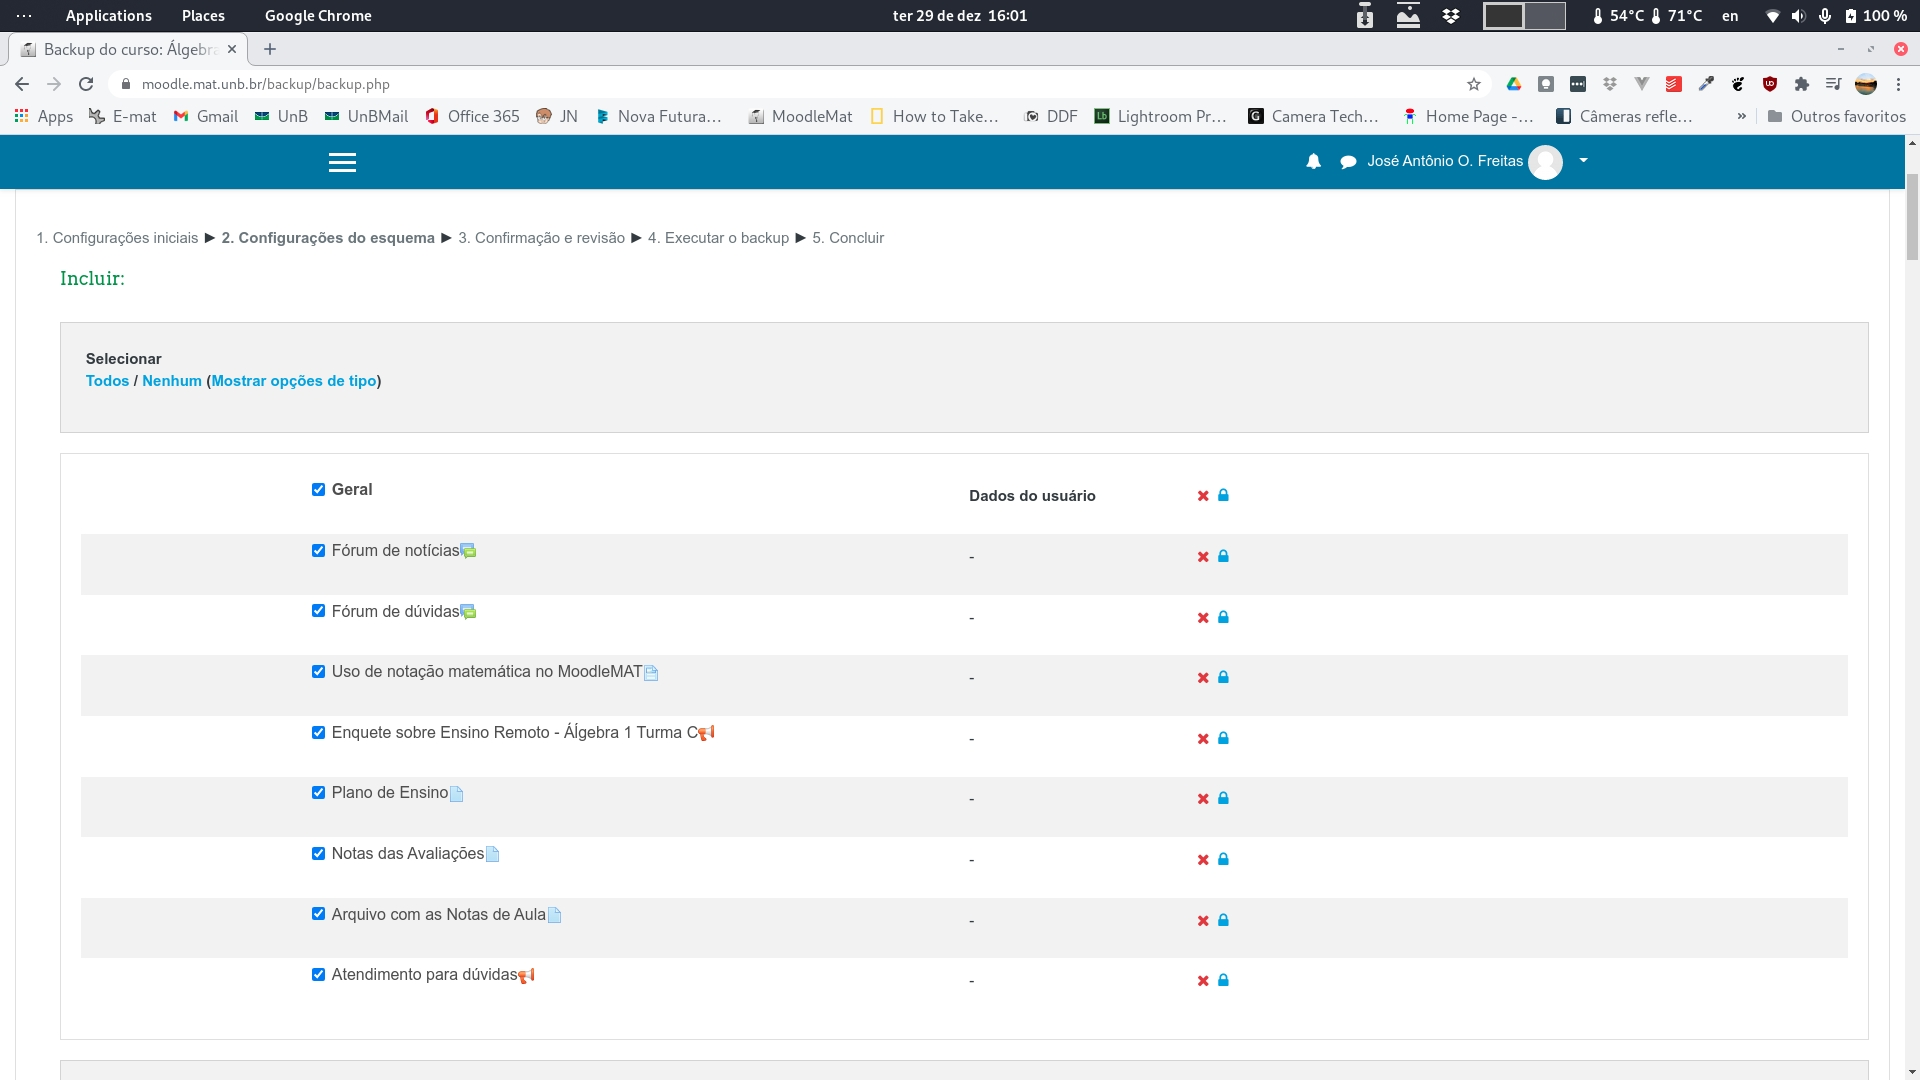
\includegraphics[width = 1.4\columnwidth]{tela_backup_6.jpg}
  	\end{figure}

  	\newpage

        \item\label{final_backup} Ao final do processo clique no botão ``\textbf{CONTINUAR}'' para que você seja redicioando para a tela de download o arquivo de backup.
	\begin{figure}[H]
    	\centering
    	\hspace*{-2.5cm}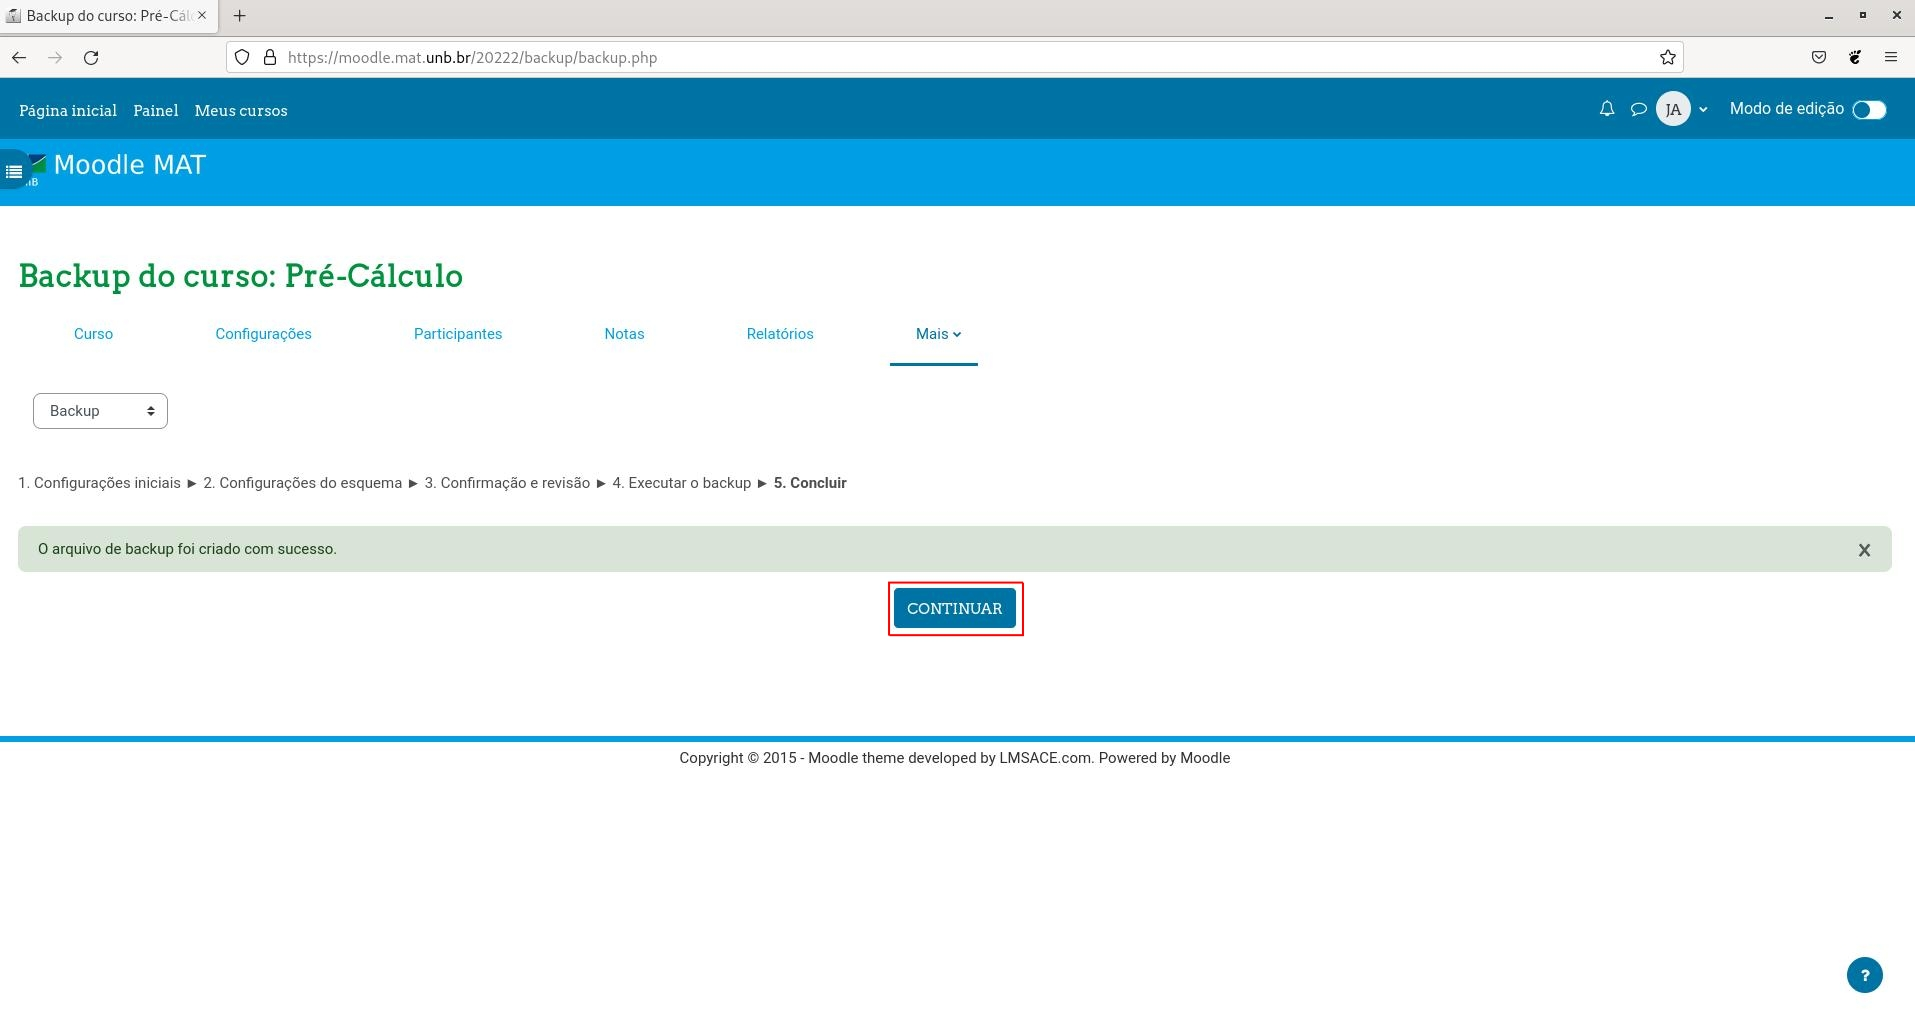
\includegraphics[width = 1.4\columnwidth]{tela_backup_10.jpg}
  	\end{figure}

  	\newpage

        \item Na página que se abre procure o texto "\textbf{Área de backup de arquivos privados do usuário}''. É nessa seção que se encotram os backups realizaros. Encontre o arquivo que deseja baixar e clique no botão ``\textbf{Download}''.
	\begin{figure}[H]
	   \centering
	   \hspace*{-2.5cm}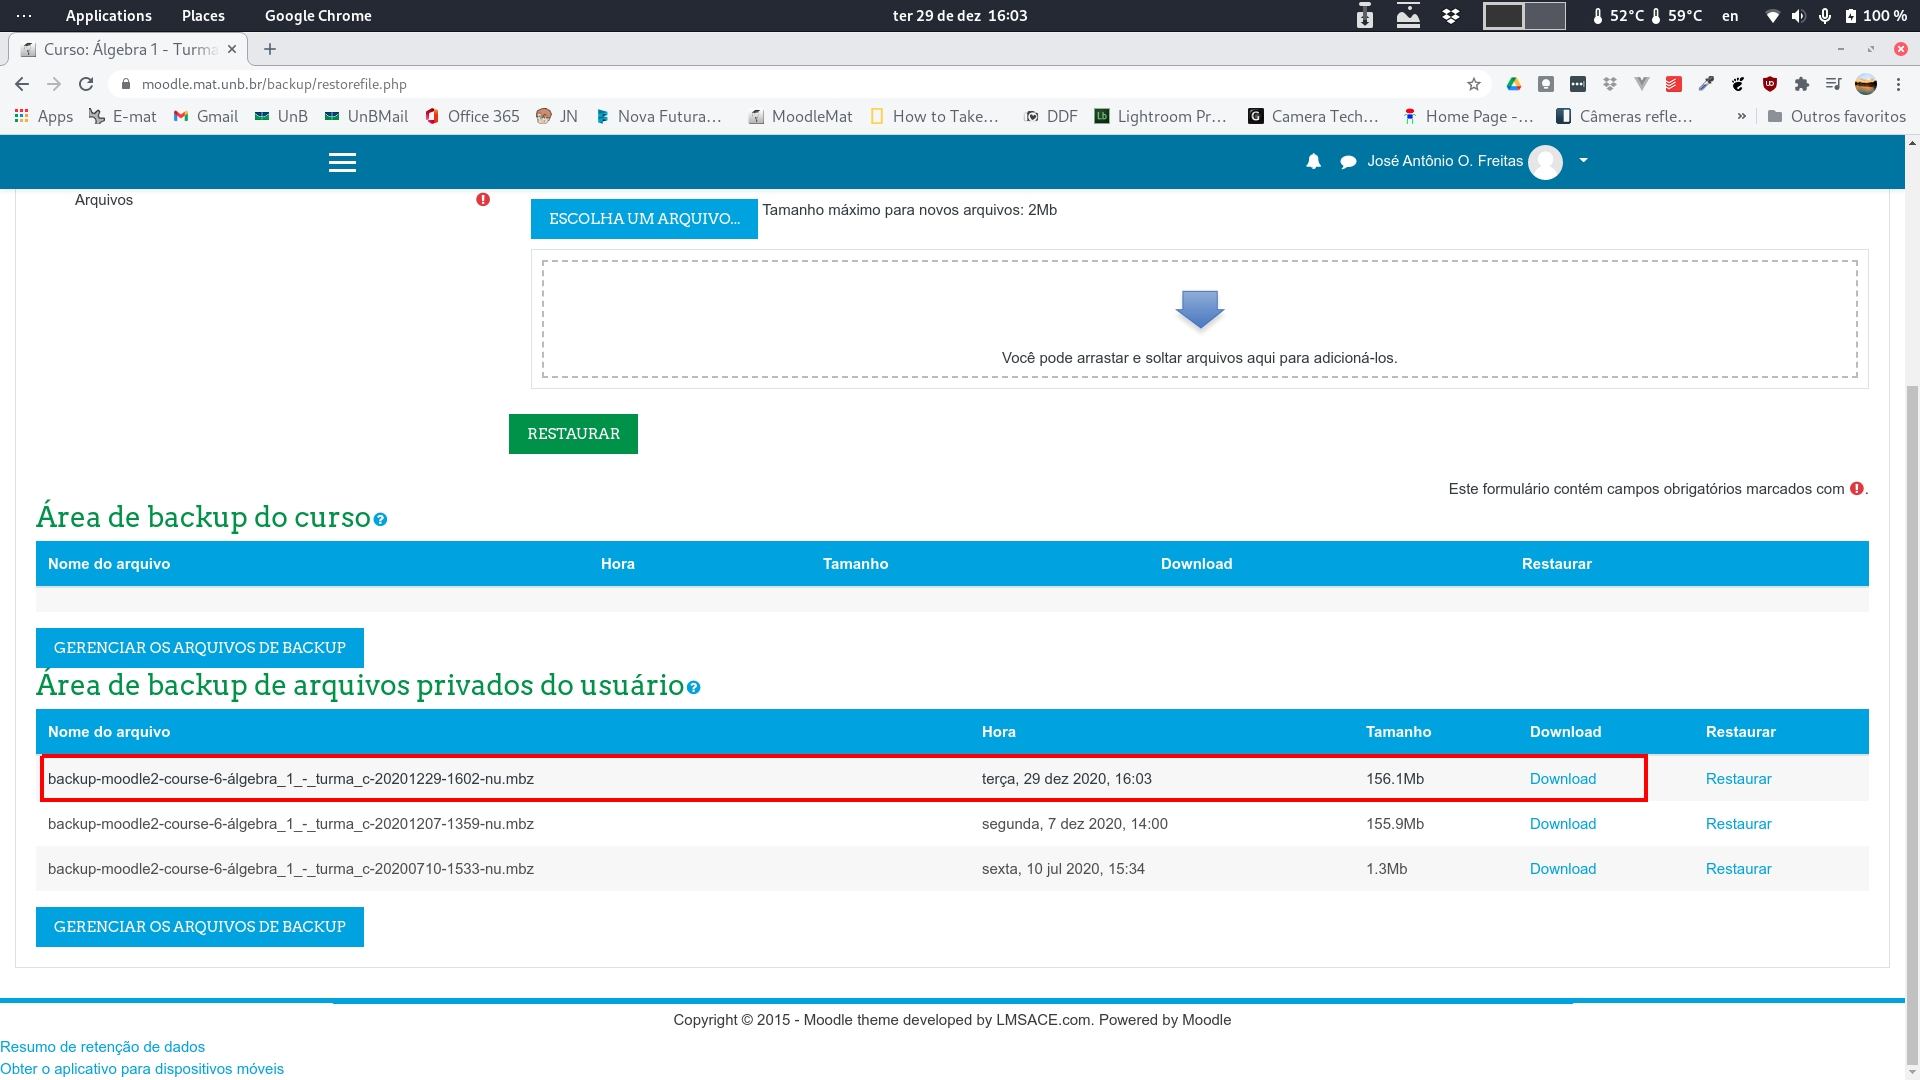
\includegraphics[width = 1.4\columnwidth]{tela_backup_11.jpg}
  	\end{figure}
\end{enumerate}

\newpage
\begin{center}
{\Large \textbf{Tutorial para a realiza\c{c}\~ao de restauração de disciplinas no MoodleMAT}}
\end{center}

\vspace{.3cm}

\hrule

\vspace{.7cm}
Para restaurar uma disciplina antiga, \textbf{cujo backup voc\^e j\'a realizou}, realize os seguintes passos:

\begin{enumerate}[\bf 1)]
	\item Ap\'os entrar na sua disciplina, no menu que aparece logo abaixo do nome da sua disciplina, clique na opção ``\textbf{Mais}''.
	\begin{figure}[H]
    	\centering
    	\hspace*{-2.5cm}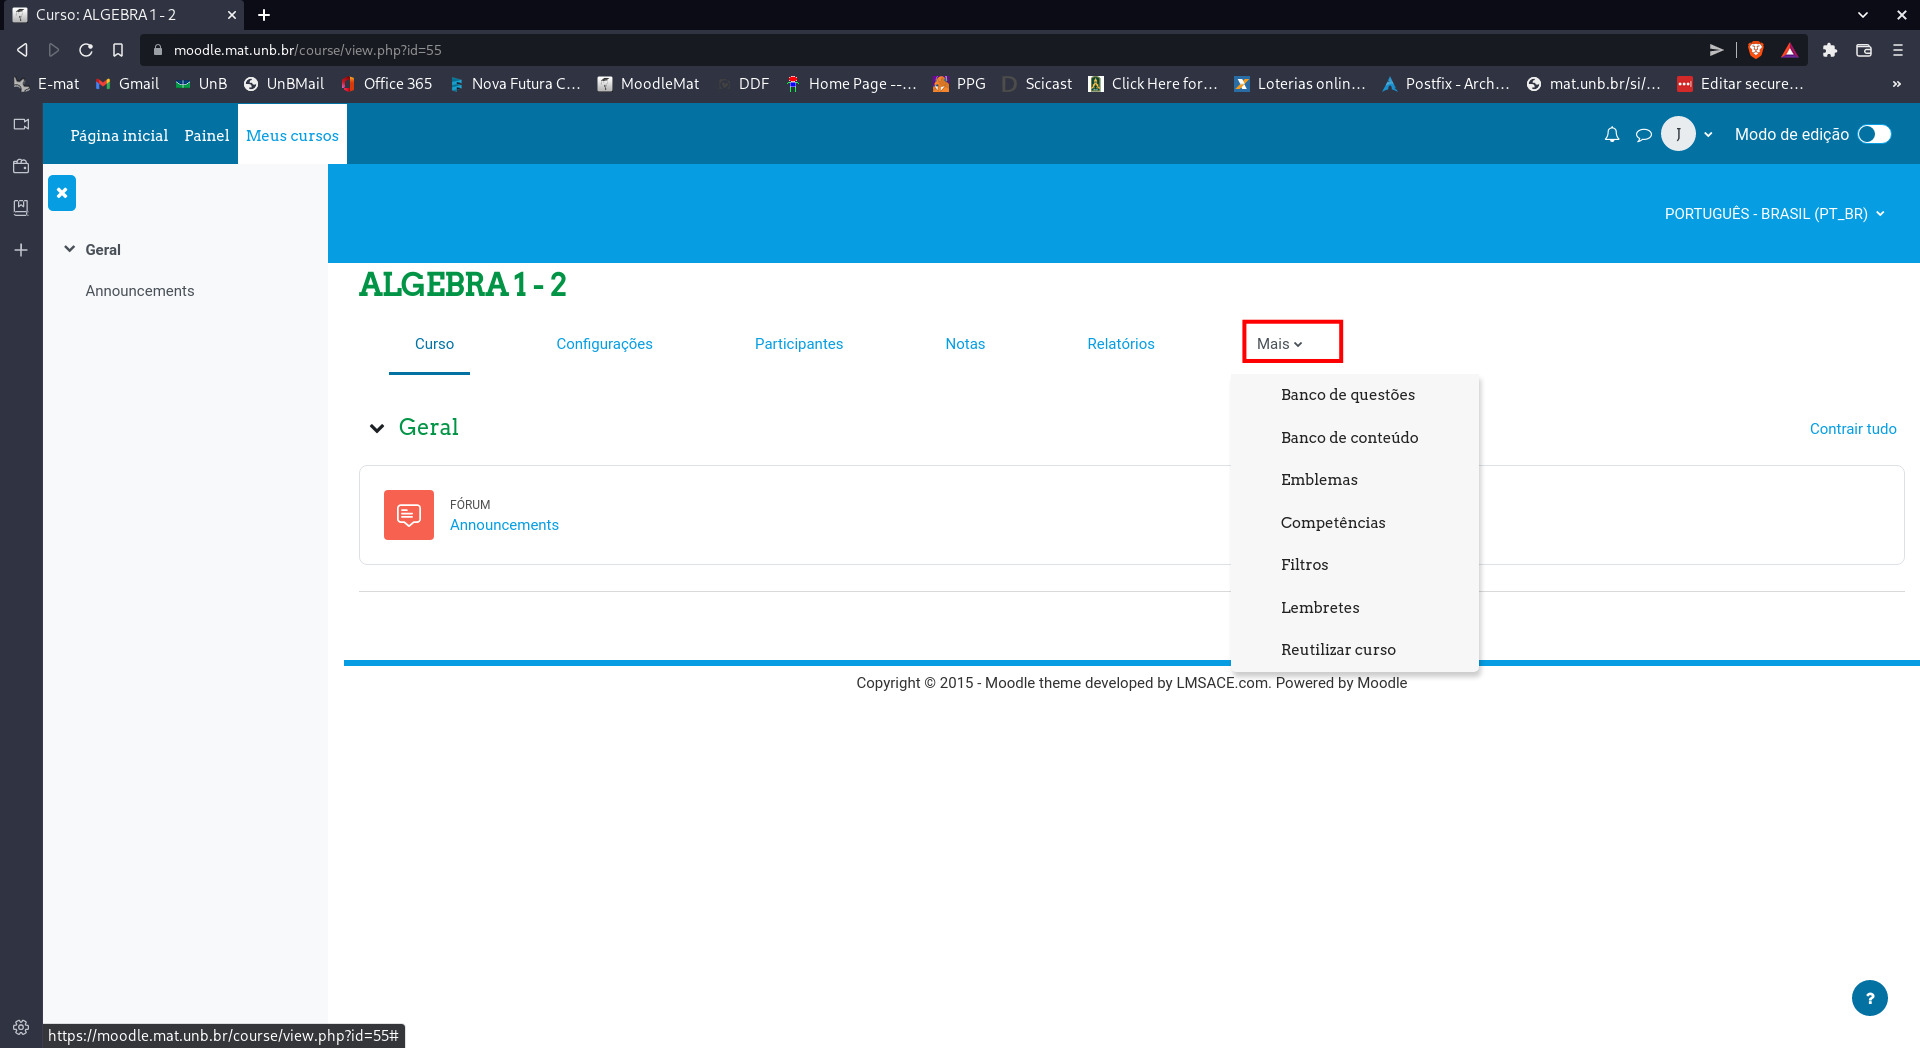
\includegraphics[width = 1.4\columnwidth]{tela_restauracao_1.jpg}
  	\end{figure}

  	\newpage

	\item No menu que abrirá clique na opção ``\textbf{Reutilizar curso}''.
	\begin{figure}[H]
    	\centering
    	\hspace*{-2.5cm}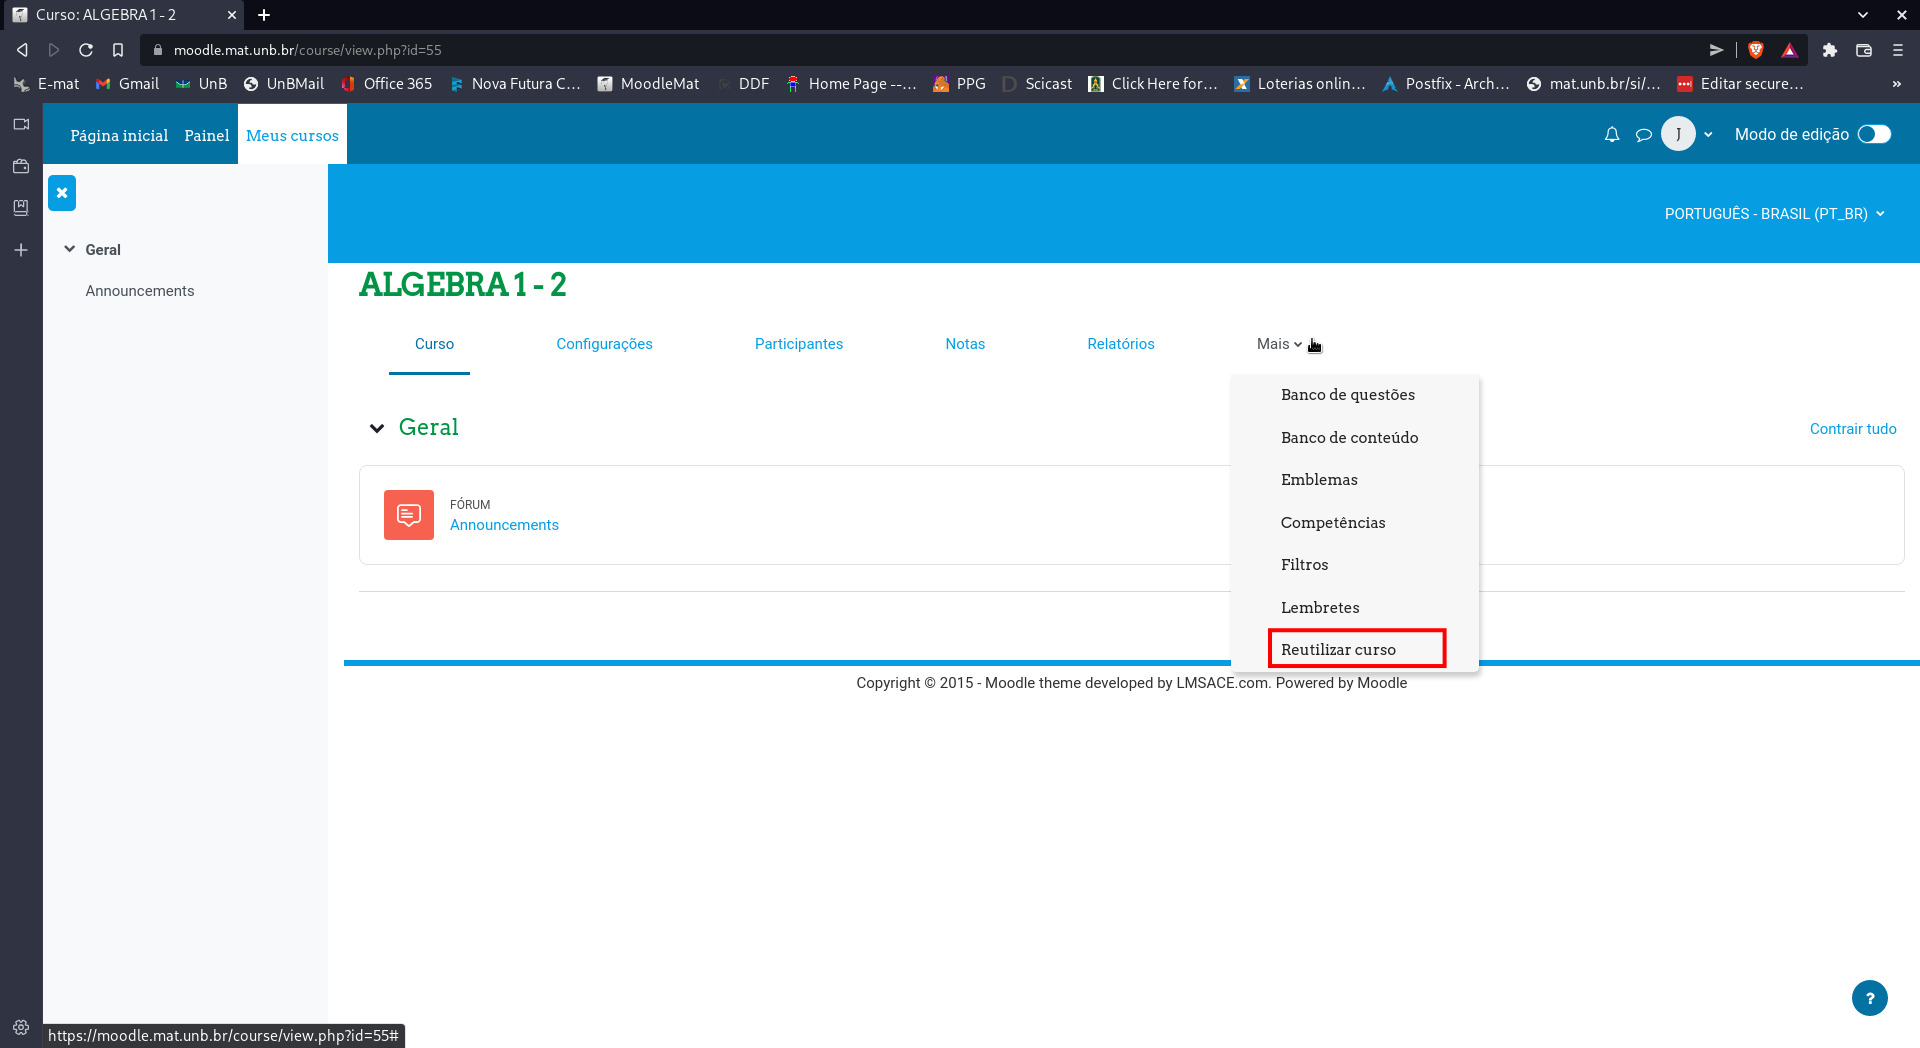
\includegraphics[width = 1.4\columnwidth]{tela_restauracao_reutilizar_curso.jpg}
  	\end{figure}

  	\newpage

    \item Na tela que será apresentada, no lado esquerdo procure um menu que conterá o texto ``\textbf{Importar}'' e clique nessa opção.
	\begin{figure}[H]
    	\centering
    	\hspace*{-2.5cm}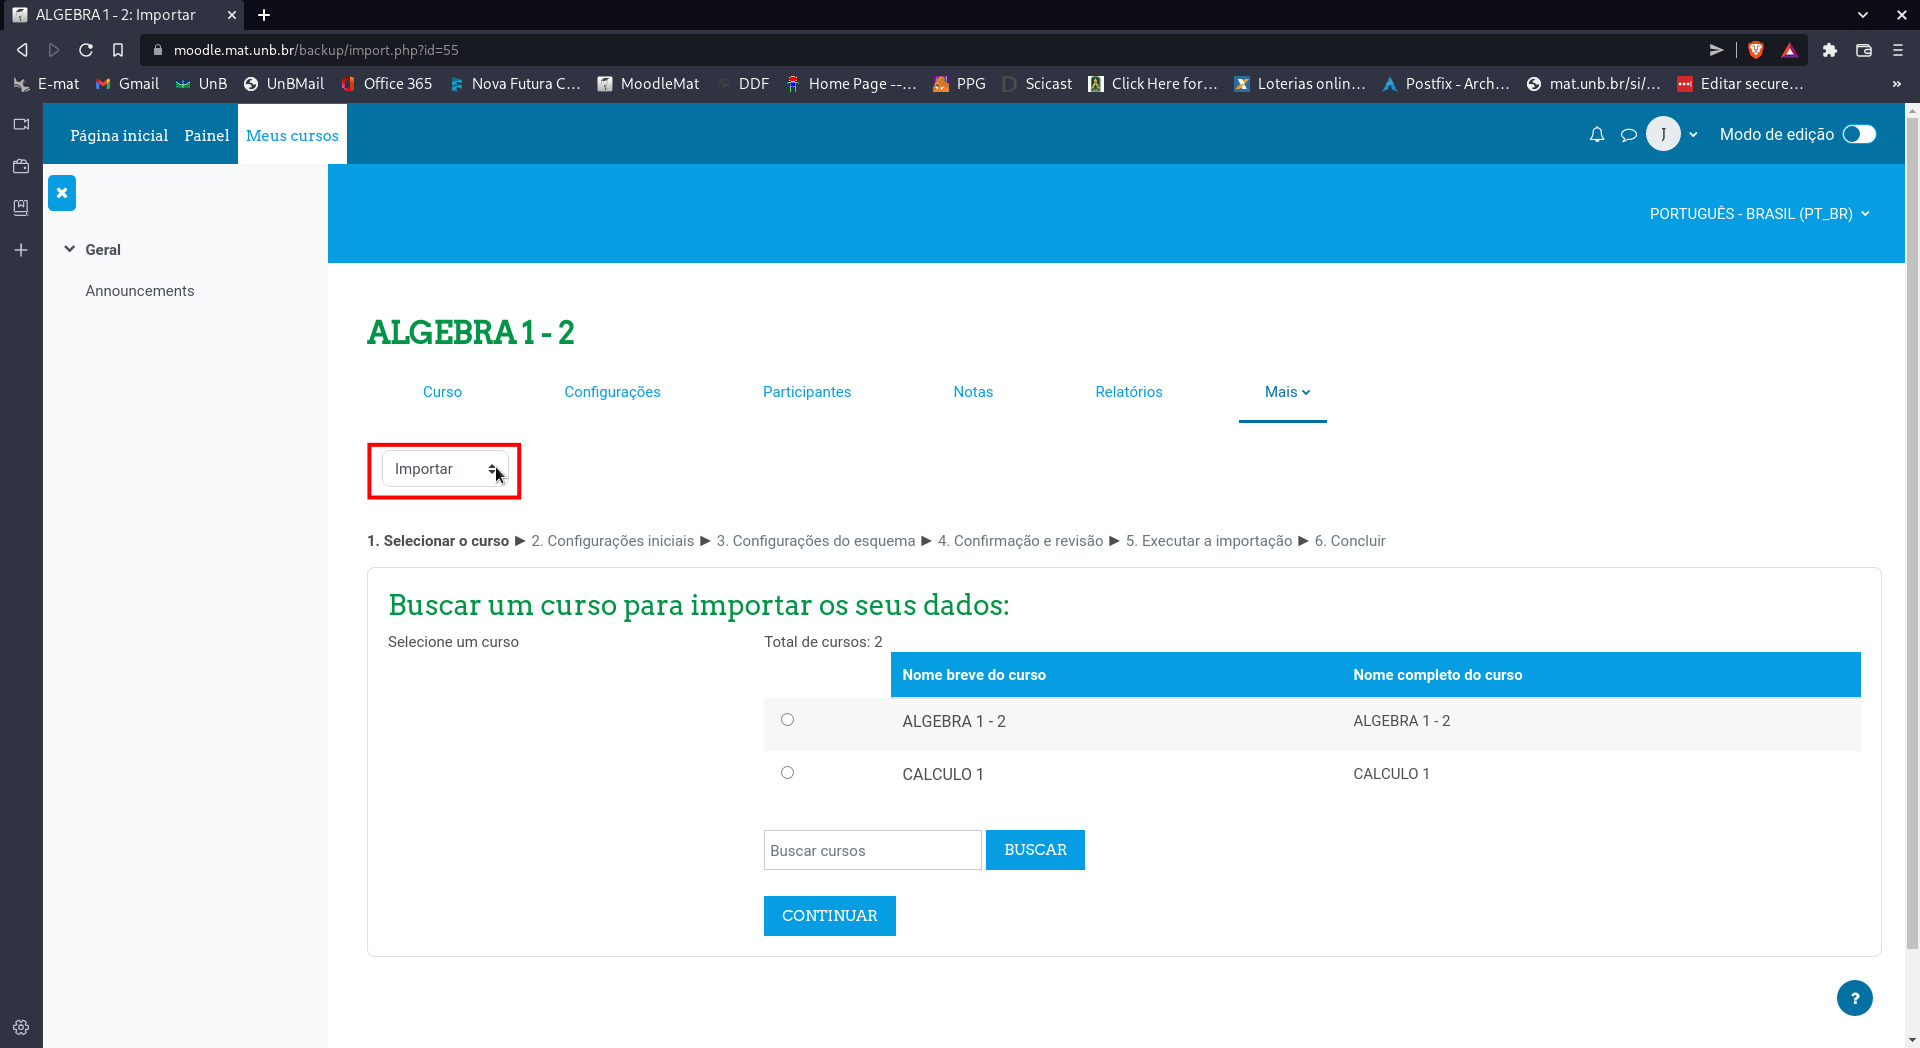
\includegraphics[width = 1.4\columnwidth]{tela_restauracao_menu_restauracao.jpg}
  	\end{figure}

  	\newpage

    \item No menu que se abrirá procure a opção ``\textbf{Restaurar}'' e clique nessa opção.
	\begin{figure}[H]
    	\centering
    	\hspace*{-2.5cm}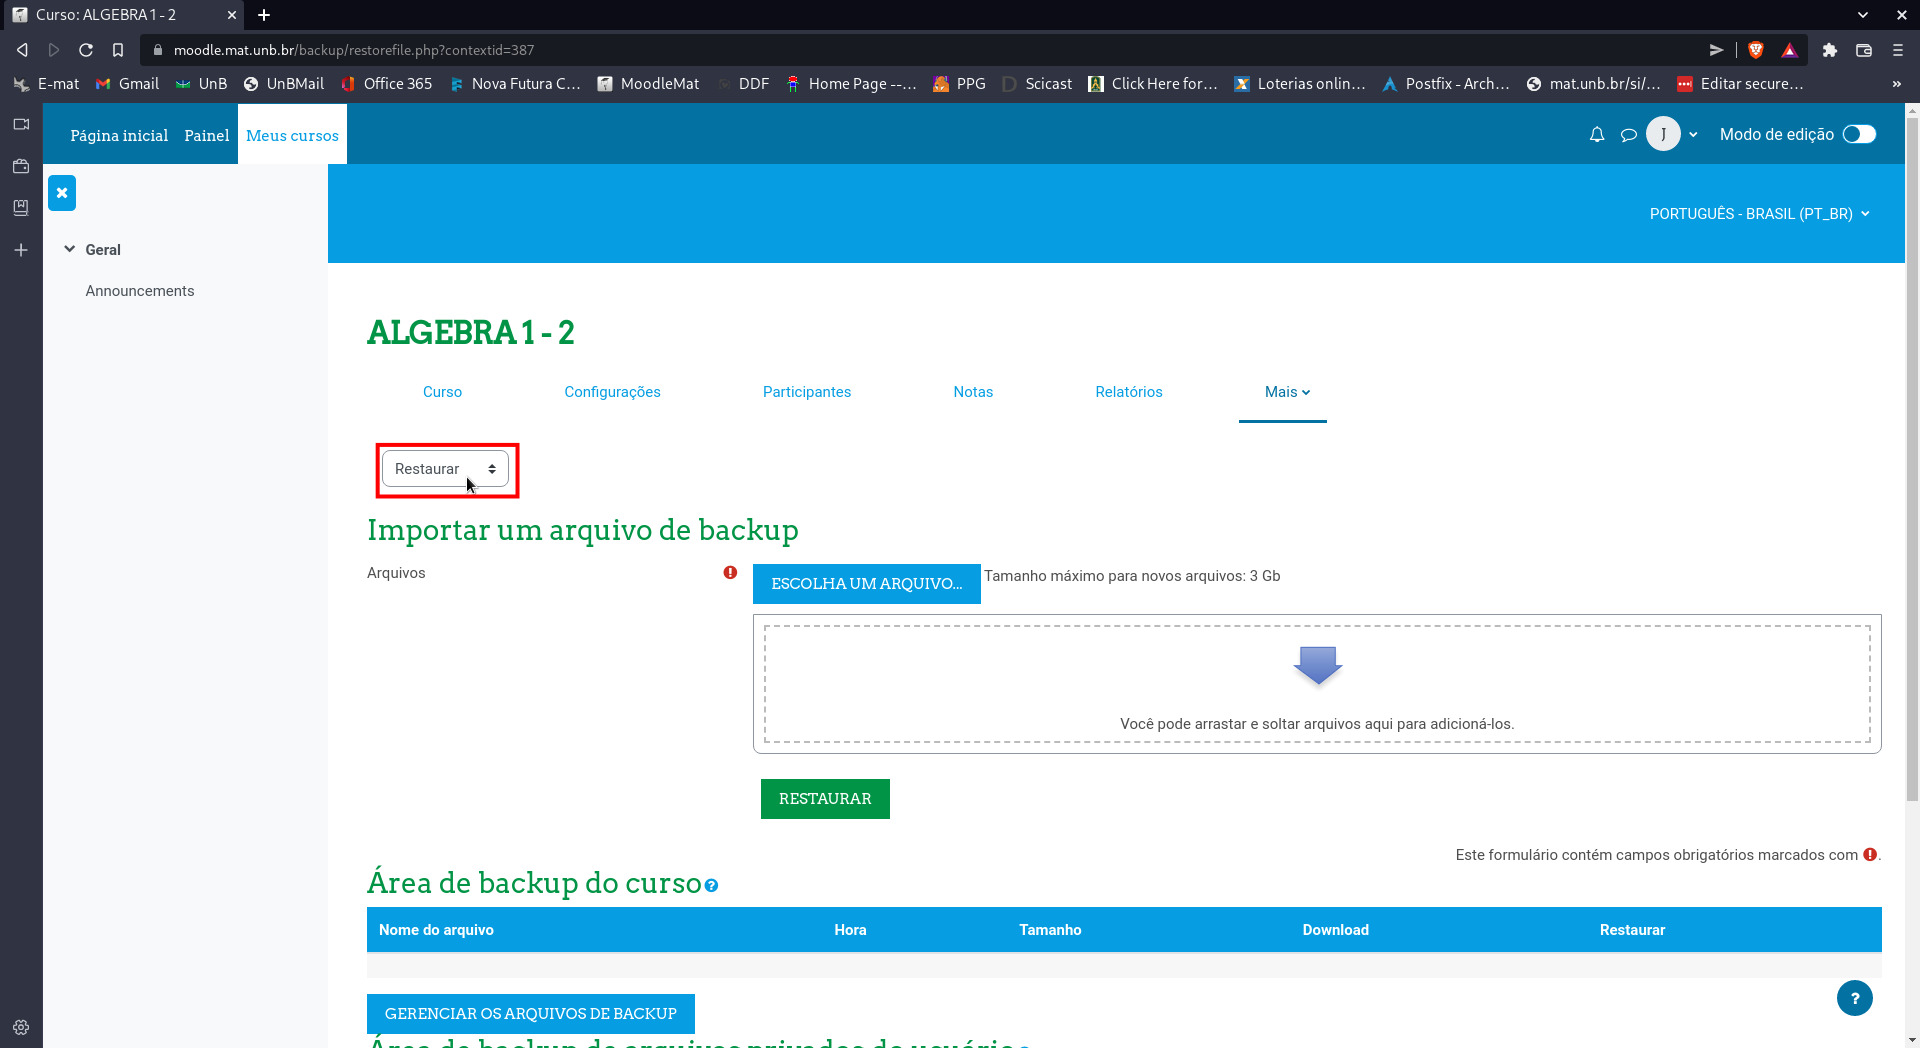
\includegraphics[width = 1.4\columnwidth]{tela_restauracao_menu_restaurar.jpg}
  	\end{figure}

  	\newpage


	\item Na pr\'oxima tela, utilize o bot\~ao ``ESCOLHA UM ARQUIVO'' para enviar o arquivo com o backup de seu curso. O processo de upload pode demorar devido ao tamanho do arquivo, velocidade de sua conex\~ao e fatores que possam estar afetando a rede da UnB.
	\begin{figure}[H]
    	\centering
    	\hspace*{-2.5cm}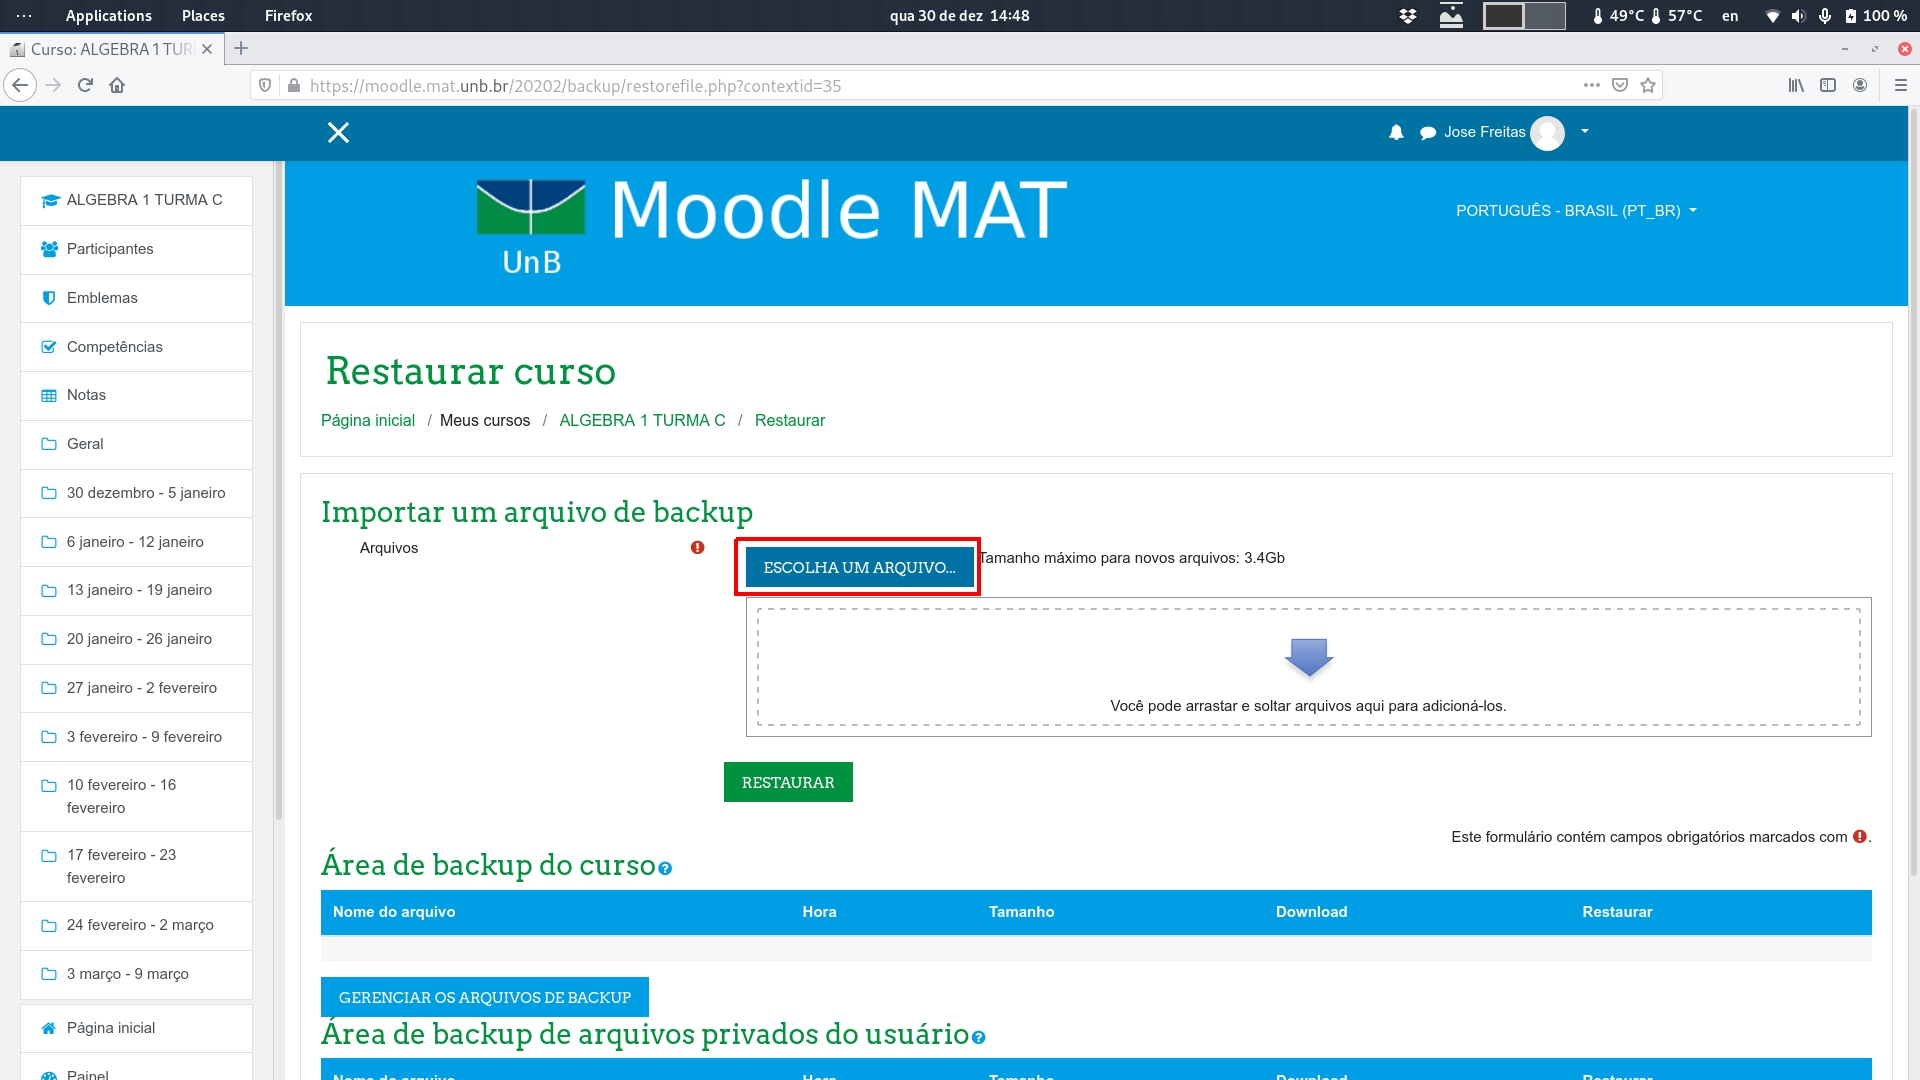
\includegraphics[width = 1.4\columnwidth]{tela_restauracao_4.jpg}
  	\end{figure}

  	\newpage

	\item Ap\'os a finaliza\c{c}\~ao do upload do arquivo voc\^e ser\'a direcionado para a tela abaixo. Clique no bot\~ao ``RESTAURAR''.
	\begin{figure}[H]
    	\centering
    	\hspace*{-2.5cm}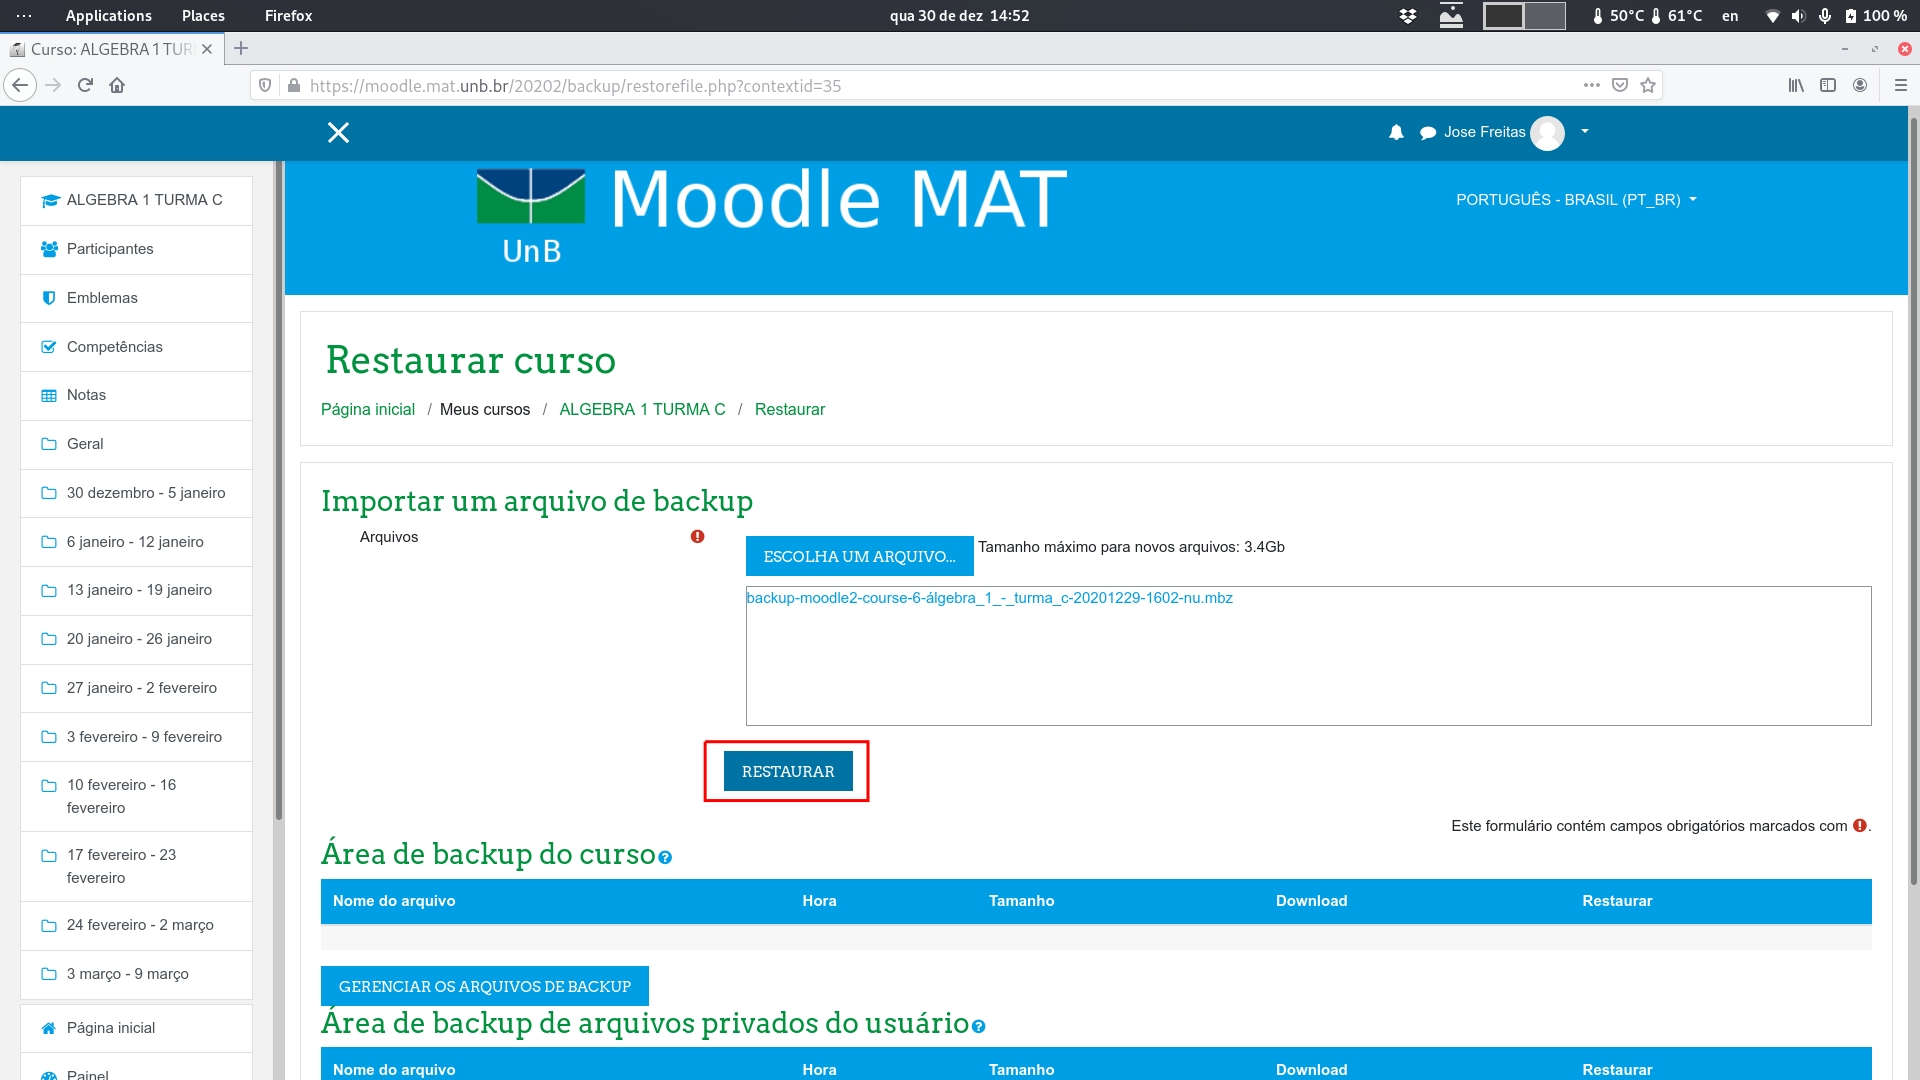
\includegraphics[width = 1.4\columnwidth]{tela_restauracao_5.jpg}
  	\end{figure}

	\newpage

	\item  Na tela que ser\'a carregada voc\^e ver\'a algumas informa\c{c}\~oes sobre os dados que ser\~ao restaurados. Navegue at\'e o final da p\'agina e clique no bot\~ao ``PR\'OXIMO''.
	\begin{figure}[H]
    	\centering
    	\hspace*{-2.5cm}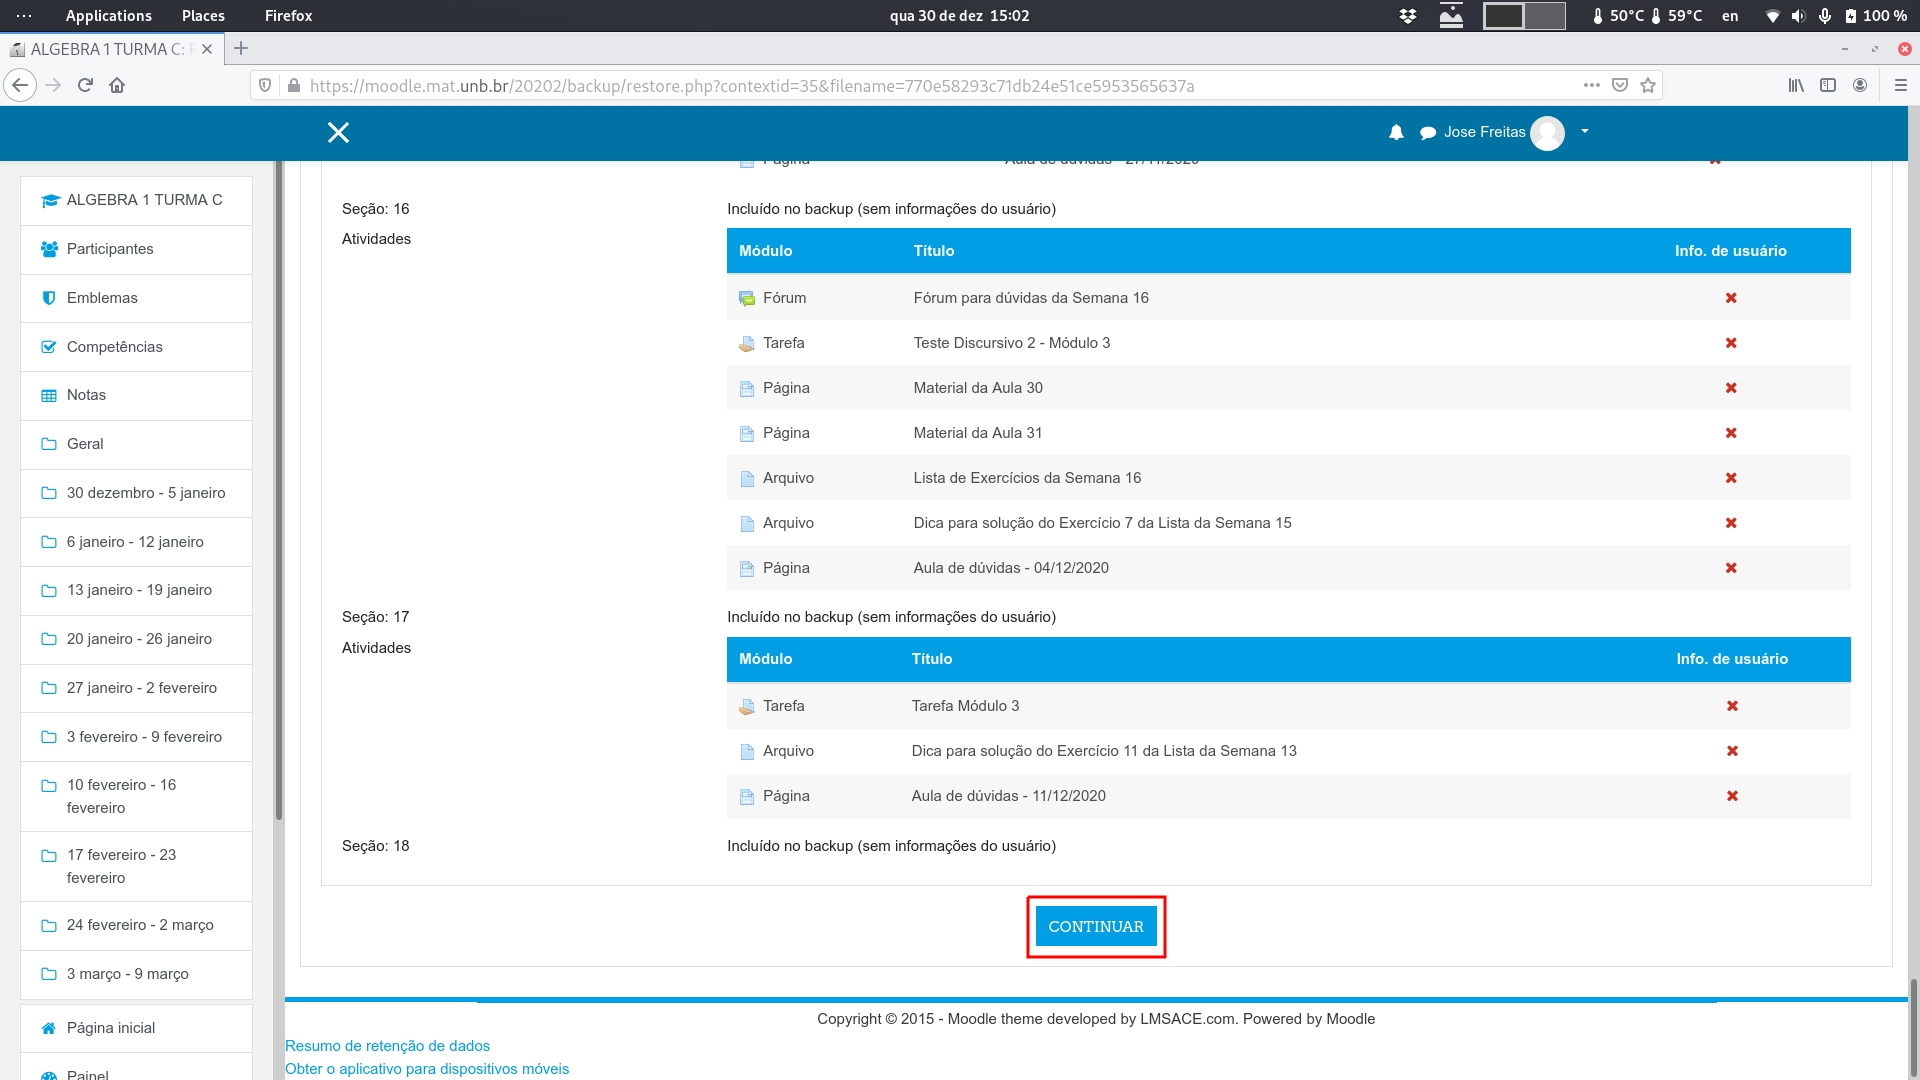
\includegraphics[width = 1.4\columnwidth]{tela_restauracao_7.jpg}
  	\end{figure}

  	\newpage

	\item Na pr\'oxima tela procure o campo ``\textbf{Restaura neste curso}'' e marque a op\c{c}\~ao ``\textbf{Excluir o conte\'udo deste curso e restaurar o backup}''. Ap\'os isso clique no bot\~ao ``CONTINUAR''.
	\begin{figure}[H]
    	\centering
    	\hspace*{-2.5cm}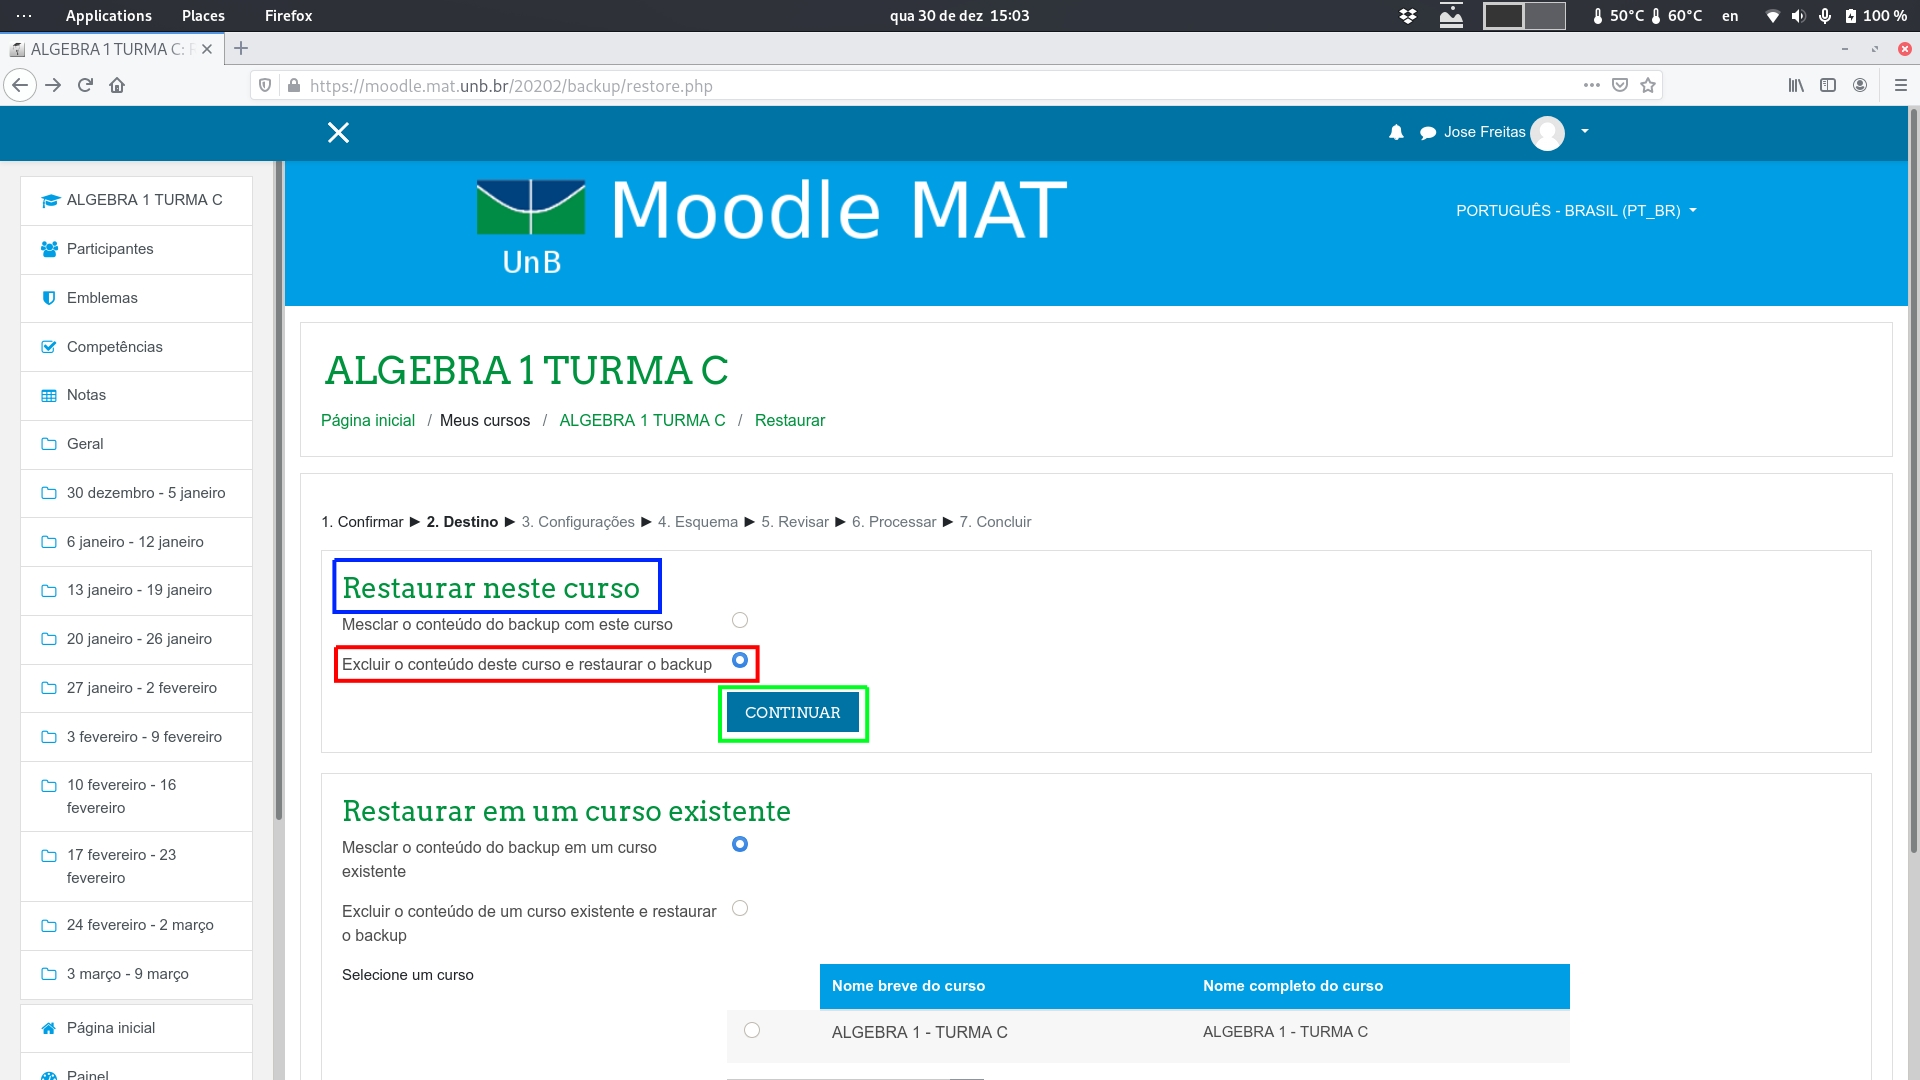
\includegraphics[width = 1.4\columnwidth]{tela_restauracao_8.jpg}
  	\end{figure}

	\newpage

	\item Na pr\'oxima tela des\c{c}a at\'e o final da p\'agina e clique em ``PR\'OXIMO''.
	\begin{figure}[H]
    	\centering
    	\hspace*{-2.5cm}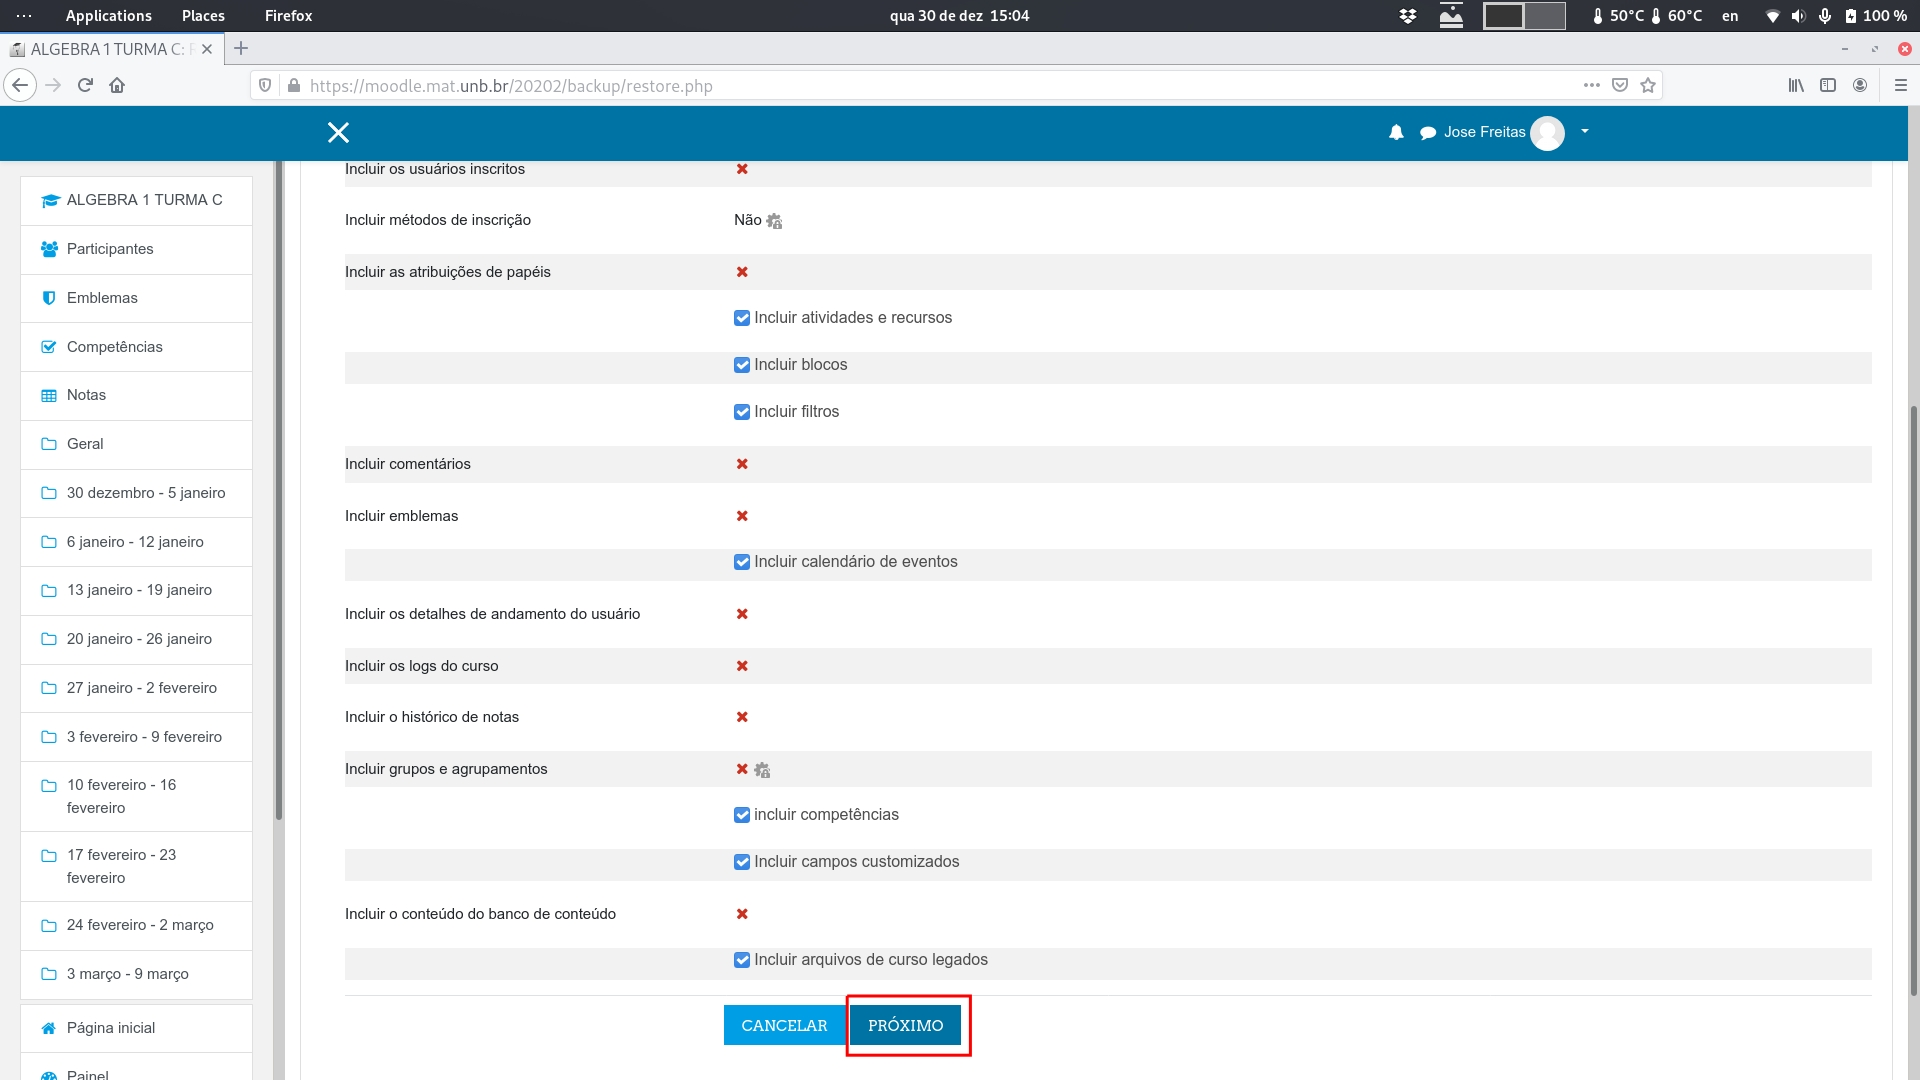
\includegraphics[width = 1.4\columnwidth]{tela_restauracao_9.jpg}
  	\end{figure}

  	\newpage

	\item Na tela seguinte ser\'a poss{\'\i}vel remover algum conte\'udo que julgar que sua restaura\c{c}\~ao n\~ao ser\'a necess\'aria. Navegue at\'e o final da p\'agina e clique em ``PR\'OXIMO''.
	\begin{figure}[H]
    	\centering
    	\hspace*{-2.5cm}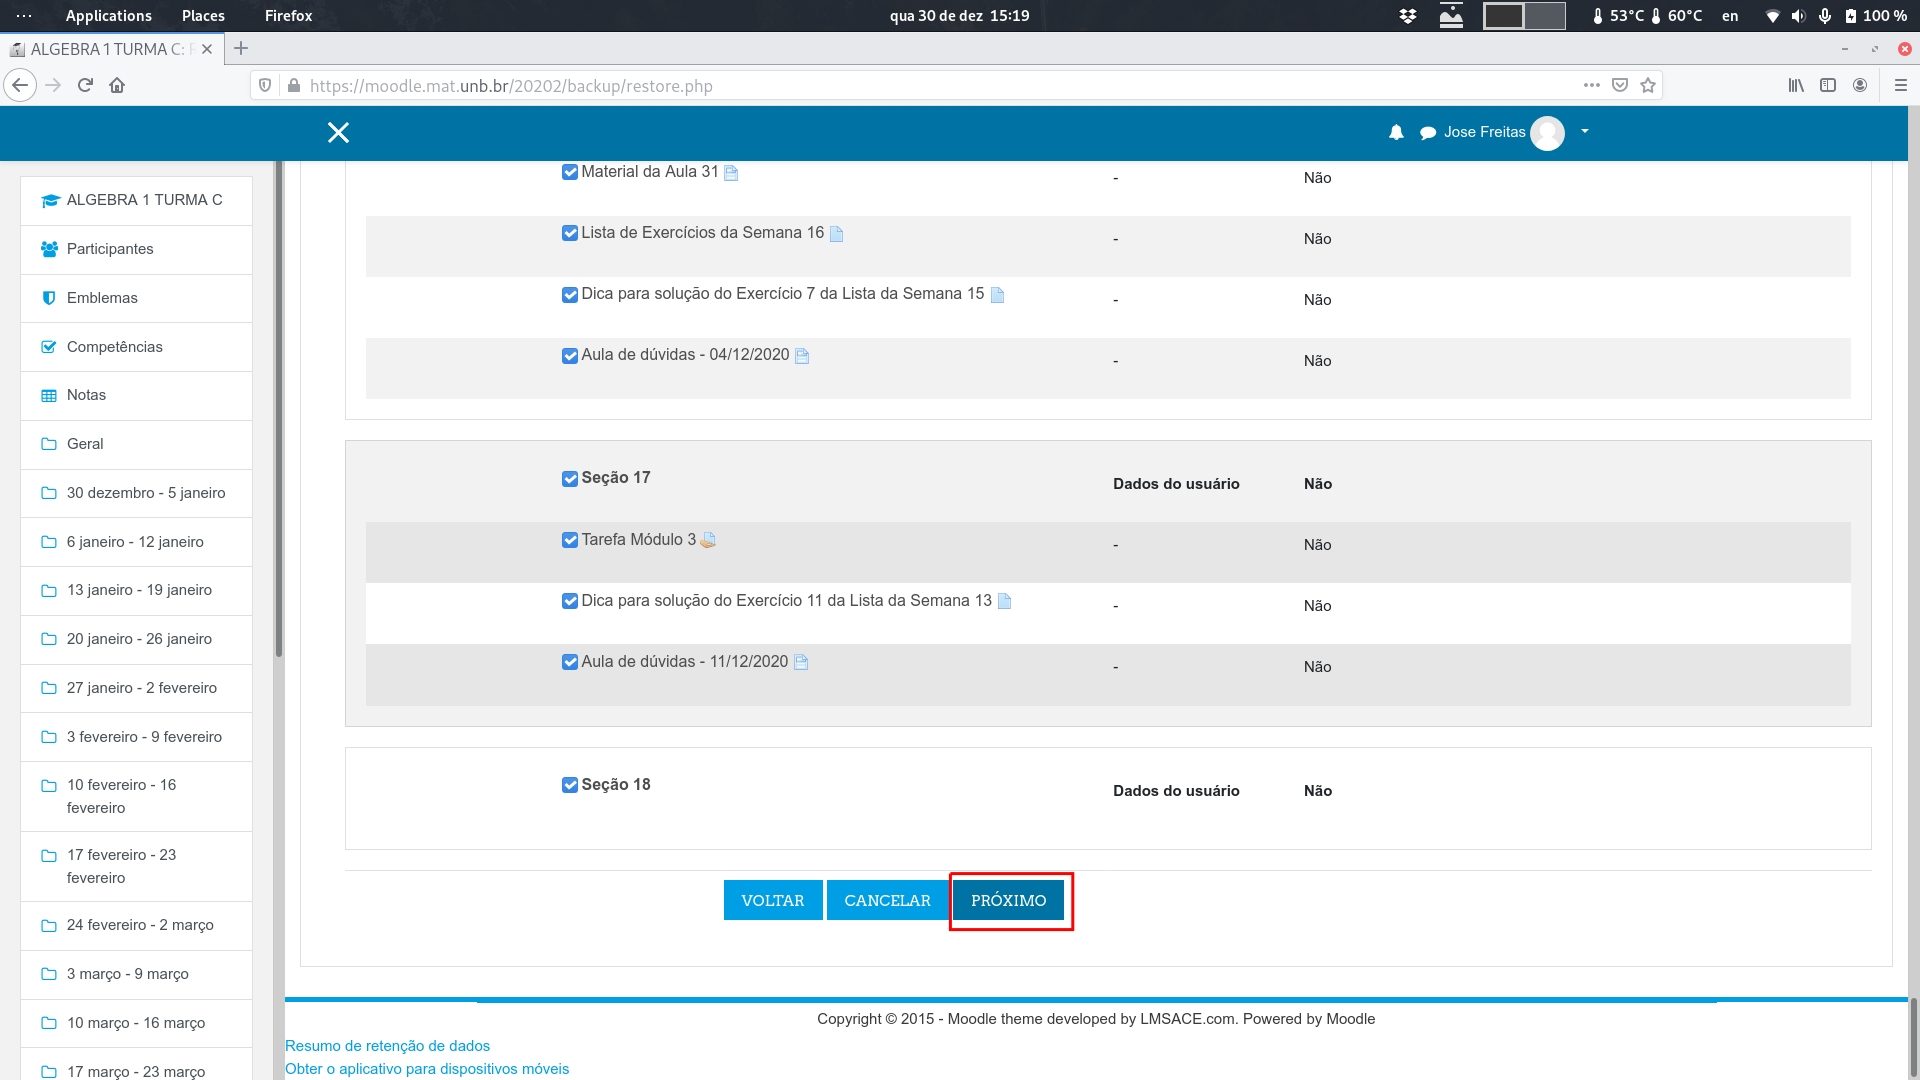
\includegraphics[width = 1.4\columnwidth]{tela_restauracao_11.jpg}
  	\end{figure}

	\newpage

	\item Na tela seguinte ser\'a apresentado um resumo dos dados que ser\~ao restaurados. Navegue at\'e o final da p\'agina e clique em ``EXECUTAR A RESTAURA\c{C}\~AO''.
	\begin{figure}[H]
    	\centering
    	\hspace*{-2.5cm}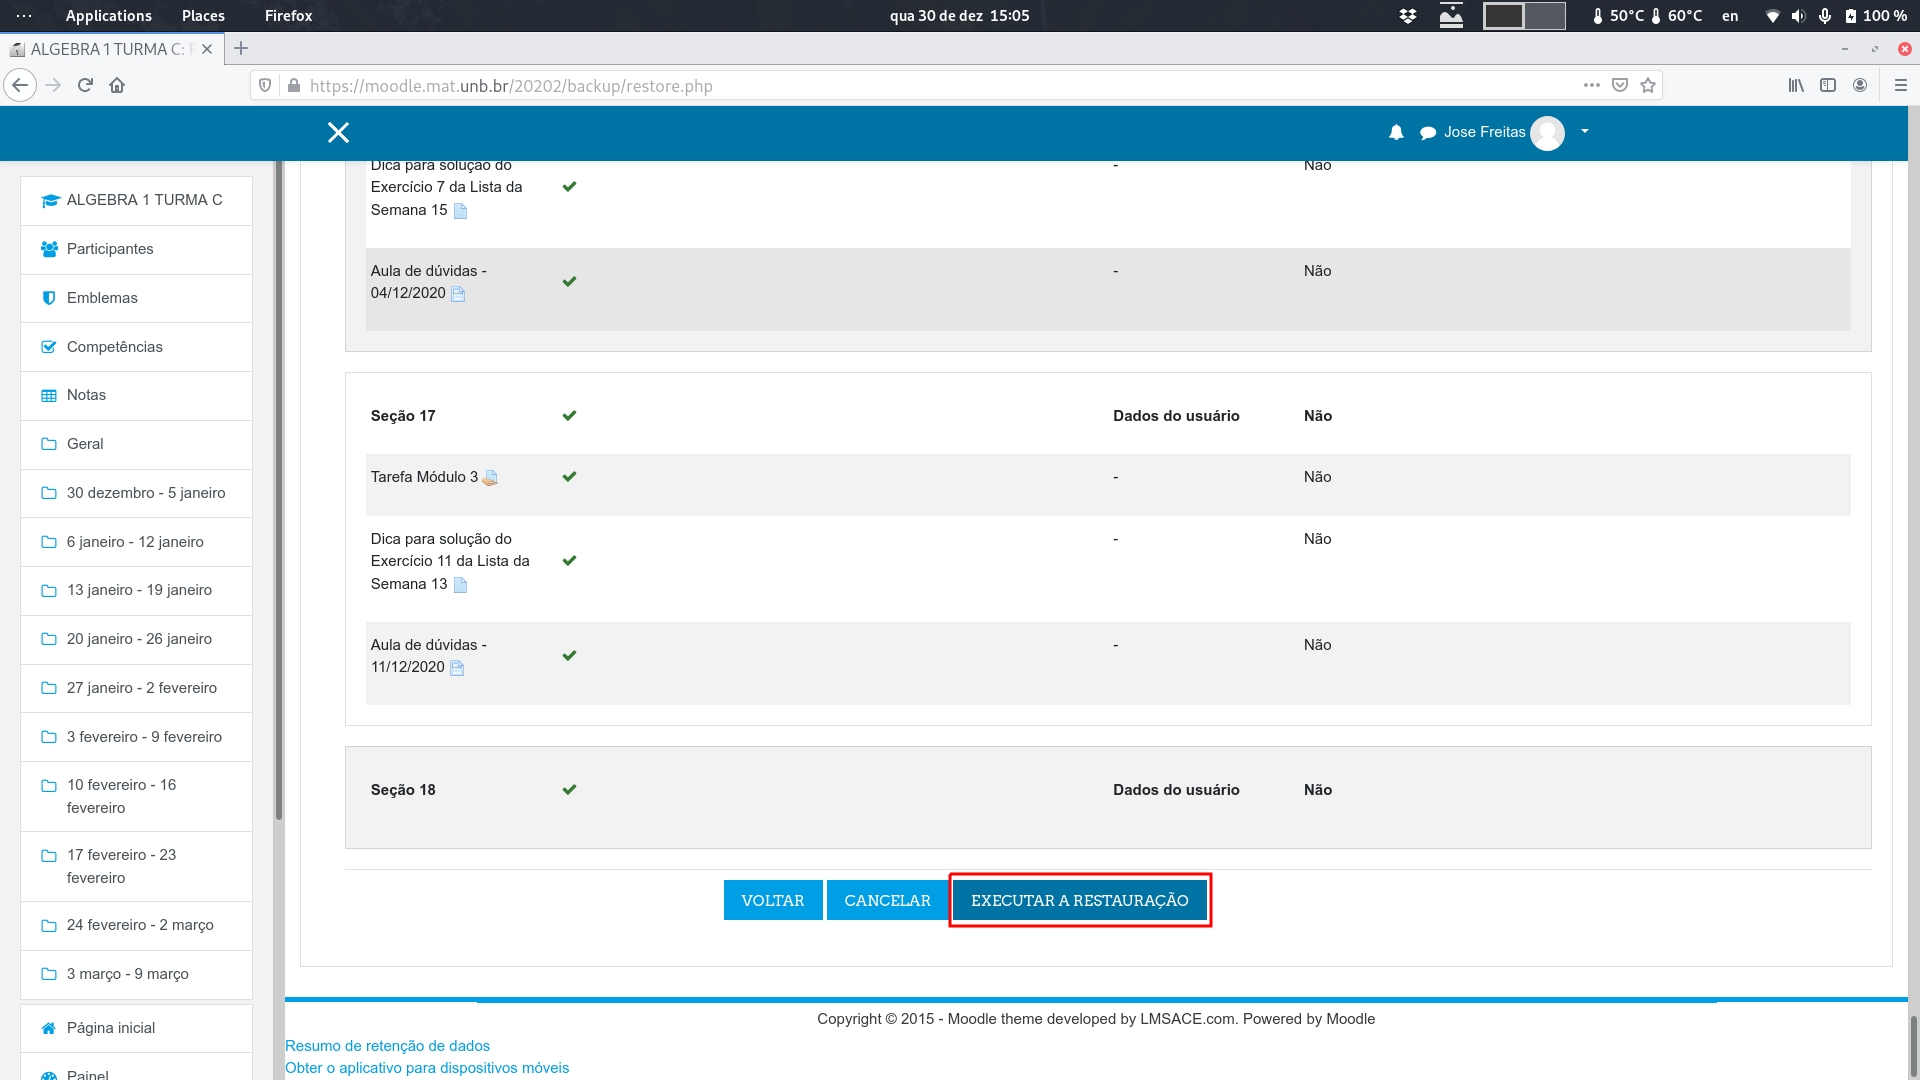
\includegraphics[width = 1.4\columnwidth]{tela_restauracao_12.jpg}
  	\end{figure}

	\newpage

	\item Ao final do processo, que poder\'a ser demorado caso a disciplina contenha muito conte\'udo, voc\^e ser\'a direcionado \`a tela final. Clicando em ``CONTINUAR'' voc\^e ser\'a enviado para a p\'agina inicial do MoodleMAT com a sua disciplina restaurada.
	\begin{figure}[H]
    	\centering
    	\hspace*{-2.5cm}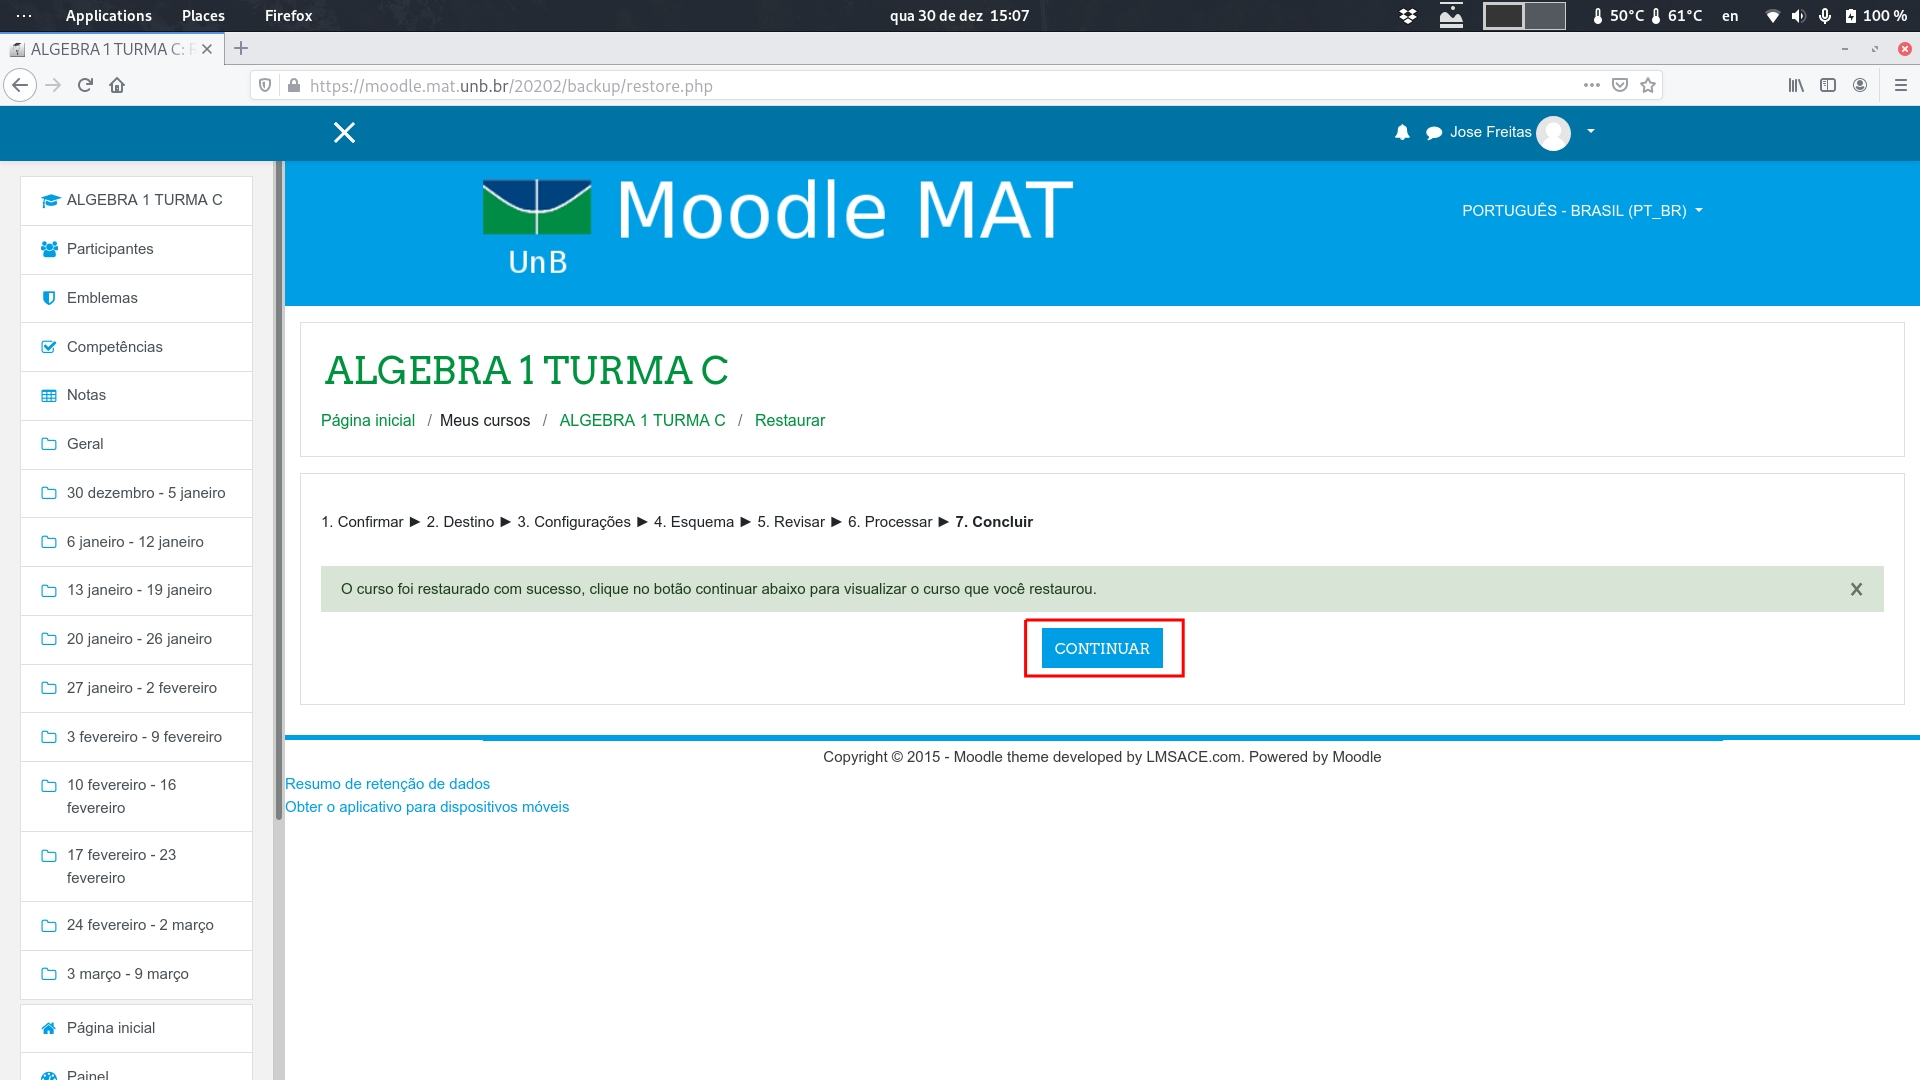
\includegraphics[width = 1.4\columnwidth]{tela_restauracao_13.jpg}
  	\end{figure}
\end{enumerate}
\end{document}
